\documentclass[12pt, a4paper]{article}

\usepackage[margin=1in, headheight=15pt]{geometry}
\usepackage{graphicx}
\usepackage{titlesec}
\usepackage{enumitem}
\usepackage{hyperref}
\usepackage{booktabs}
\usepackage{array}
\usepackage{parskip}
\usepackage{setspace}
\usepackage{fancyhdr}
\usepackage{xcolor}
\usepackage{float}
\usepackage{amsmath}
\usepackage{amssymb}
\usepackage{tabularx}
\usepackage{colortbl}

\hypersetup{
    colorlinks=true,
    linkcolor=black,
    urlcolor=blue,
    citecolor=black
}

\pagestyle{fancy}
\fancyhf{}
\rhead{\textit{\textcolor{orange}{UniConnecT}}}
\lhead{\textit{System Analysis and Design --- UIU}}
\rfoot{\thepage}
\renewcommand{\headrulewidth}{0.4pt}

\titleformat{\section}{\large\bfseries}{\thesection.}{0.5em}{}
\titleformat{\subsection}{\normalsize\bfseries}{\thesubsection}{0.5em}{}

\setlist[itemize]{itemsep=2pt, topsep=4pt}
\setlist[enumerate]{itemsep=2pt, topsep=4pt}

\onehalfspacing

% ---------------------------------------------------------------
\begin{document}

% ---------------------------------------------------------------
%  COVER PAGE
% ---------------------------------------------------------------
\begin{titlepage}
    \centering
    \vspace*{0.6cm}
    
    
    {\Huge \textbf{Software Requirements Specification (SRS)}}\\[0.4cm]
    
\includegraphics[width=0.55\textwidth, height=0.20\textheight, keepaspectratio]{Logo Final Big.png}
    
    
    {\large \textit{A Private University Social Network Platform}}\\[0.25cm]
    \rule{\textwidth}{1pt}\\[0.9cm]

    {\large \textbf{Prepared by --- Team Mavericks:}}\\[0.3cm]

    \begin{tabular}{ll}
        \toprule
        \textbf{Name} & \textbf{Student ID} \\
        \midrule
        {Joydip Datta}                      & {0112330960} \\
        {MD. Saem Ferdous}                  & {0112330950} \\
        {Md. Monabbur Hosen Bhuiyan}        & {0112330936} \\
        {Md. Mahfujur Rahman Himel Akon}    & {0112330935} \\
        \bottomrule
    \end{tabular}\\[1.2cm]

    
\includegraphics[width=0.55\textwidth, height=0.20\textheight, keepaspectratio]{UIU_Logo.png}
    
    {\large \textbf{Course:} System Analysis and Design}\\[0.15cm]
    {\large \textbf{Institution:} United International University (UIU), Dhaka}\\[0.15cm]
    {\large \textbf{Submission Date:} 17 June 2026}\\[1cm]
    


    

    

    \vfill
\end{titlepage}

% ---------------------------------------------------------------
\tableofcontents
\newpage

% ---------------------------------------------------------------
\section{Introduction}
% ---------------------------------------------------------------

\subsection{Project Overview}

UniConnecT is a multi-tenant private social networking platform designed exclusively for
university communities, connecting students, alumni, faculty, and administrative staff
within a shared, institution-specific digital environment. Unlike general-purpose social
networks, UniConnecT scopes all interactions, content, and connections to a single
university per deployment, ensuring every engagement is relevant, verified, and
community-driven. The platform serves as a central hub for academic and professional
campus life, bringing together social engagement, career opportunities, mentorship,
campus services, and real-time communication under one cohesive interface.

\subsection{Purpose of the System}

The purpose of UniConnecT is to eliminate the fragmentation that currently exists across
university communication channels by providing one cohesive platform where every member
of the university community can connect, collaborate, and grow. Through UniConnecT,
students can build their professional network, discover job and internship opportunities,
receive structured mentorship from alumni, stay informed through official university news,
join groups and clubs, and coordinate campus activities --- all within a verified,
institution-bound environment. Faculty and administrators gain a structured channel to
publish announcements, manage users and content, and engage with the broader campus
community. Transport staff can broadcast live shuttle location data for student use.

\subsection{Problem Statement / Motivation}

University communities currently lack a dedicated digital space that serves their unique
social and professional needs. Students rely on a fragmented combination of general social
media platforms, university email chains, physical notice boards, and third-party job
portals --- none of which are tailored to the university context or integrated with one
another. This fragmentation results in missed job and internship opportunities, weak
alumni-to-student mentorship pipelines, poor information flow between administration and
students, and no unified sense of campus identity online. Beyond social and professional
concerns, practical campus services such as lost-and-found coordination and shuttle
tracking are handled through informal channels with no digital structure. UniConnecT is
proposed to address all of these challenges by offering a modern, purpose-built platform
that brings the entire university experience --- social, professional, academic, and
logistical --- into a single, well-designed digital space.

% ---------------------------------------------------------------
\section{Project Objectives}
% ---------------------------------------------------------------

The primary objectives of UniConnecT are grouped below by theme.

\subsection{Social and Community Objectives}

\begin{itemize}
    \item \textbf{Unified Campus Social Feed:} Provide a community-driven social feed
    where students, alumni, and faculty can post, react, comment on, and share content
    relevant to their university.

    \item \textbf{Campus Events Management:} Enable creation, browsing, and RSVP for
    campus events so the community stays informed and engaged in university life.

    \item \textbf{Groups and Clubs:} Support the creation and management of university
    groups (clubs, departments, study circles) with dedicated feeds, file resources,
    study sessions, member roles, and group rules.

    \item \textbf{Real-Time Messaging:} Provide direct and group messaging for
    communication between connected community members and within mentorship relationships.
\end{itemize}

\subsection{Professional and Career Development Objectives}

\begin{itemize}
    \item \textbf{Alumni--Student Mentorship:} Design a structured mentorship module
    enabling students to discover alumni mentors and request guidance on academic and
    career development.

    \item \textbf{Job and Internship Discovery:} Offer a university-internal job board
    where alumni and faculty can post opportunities and students can browse and apply,
    all within a trusted institutional network.

    \item \textbf{Professional Connection Network:} Implement a bidirectional
    LinkedIn-style connection system allowing members to build and grow a verified
    university professional network.
\end{itemize}

\subsection{Campus Utility and Technical Objectives}

\begin{itemize}
    \item \textbf{Campus Utilities:} Integrate practical campus tools --- a
    lost-and-found item tracking module and a real-time shuttle schedule and location
    tracker --- directly into the platform.

    \item \textbf{Role-Based Access and Multi-Tenancy:} Design distinct, role-aware
    interface views for students, alumni, faculty, administrators, and transport drivers,
    with each university operating as a fully isolated tenant.

    \item \textbf{Modern, Accessible, Responsive Interface:} Deliver a visually
    consistent, accessible UI across desktop, tablet, and mobile screen sizes, built
    on a unified UIU-branded design system.
\end{itemize}

% ---------------------------------------------------------------
\section{Target Users}
% ---------------------------------------------------------------

The following user groups are the intended audience for UniConnecT. All users belong to
a single university community; the platform does not allow cross-university interaction.

\subsection{Students}

The primary users of the platform. Students use UniConnecT to browse and post on the
social feed, build connections with peers and alumni, discover jobs and internships,
join groups and clubs, RSVP for events, request mentorship from alumni, access campus
news, save drafts, report lost items, and track shuttle locations.

\subsection{Alumni}

Graduated members of the university who maintain access to the platform after leaving.
Alumni can post job and internship opportunities, offer mentorship to current students,
engage with the social feed, participate in groups, and stay professionally connected
to the university community.

\subsection{Faculty}

Academic staff members who use the platform to publish announcements and news, engage
with students and alumni, create and manage events, and participate in group
discussions. Faculty may also act in a moderation capacity within their
department-level groups.

\subsection{System Administrators}

University administrators who oversee the platform's operation. Administrators manage
user accounts and roles, issue and revoke invitation tokens, moderate reported content,
configure university-wide settings, and monitor platform activity through a dedicated
admin panel. All administrative actions are recorded in an audit log.

\subsection{Transport Drivers}

A least-privilege role assigned exclusively to campus shuttle and transport staff.
Drivers interact only with a dedicated GPS broadcast view to transmit live shuttle
location data to the platform. They have no access to the broader social application.

% ---------------------------------------------------------------
\section{Benchmark Analysis}
% ---------------------------------------------------------------

Benchmark analysis evaluates UniConnecT against the five platforms that occupy the
closest competitive space: purpose-built university alumni and community engagement
SaaS products. Unlike general social networks, these platforms are specifically sold
to higher-education institutions --- making them the most relevant frame of reference
for positioning UniConnecT's value and identifying remaining market gaps.


\subsection{Competitor Overview}

\begin{itemize}
    \item \textbf{PeopleGrove} (Direct) --- A career-success and mentoring platform
    deployed at 500+ universities primarily in the USA. PeopleGrove excels at
    structured alumni-to-student career advising and job referral workflows. However,
    it does not offer a general social feed, real-time messaging, campus utilities,
    or university news. Pricing is custom and expensive, making it inaccessible to
    South Asian institutions operating on tighter budgets.

    \item \textbf{Graduway} (Direct) --- An alumni community and engagement platform
    used by 2,750+ institutions globally. Graduway focuses on alumni directory
    management, mentorship matching, and fundraising pipelines. It is predominantly
    alumni-facing and does not serve current students, faculty, or transport staff as
    first-class actors. It lacks a social feed, real-time chat, and any campus
    utility layer. Enterprise pricing makes it prohibitive for emerging-market
    universities.

    \item \textbf{Almabase} (SaaS) --- A fundraising and events management SaaS for
    alumni associations, priced at approximately \$3,000 per year. Almabase covers
    alumni directories, giving campaigns, and event ticketing but provides no student
    social networking, job board, mentorship economy, or campus utilities.
    Its feature surface is narrow relative to its cost.

    \item \textbf{AlumnForce} (SaaS) --- A private social network for alumni
    associations, originating in Europe. AlumnForce offers alumni directories, a
    jobs board, and some social feed functionality, but the platform is alumni-only
    --- current students and faculty are not integrated as participants. Real-time
    messaging is limited. Pricing is quote-based and typically enterprise-tier,
    with little published transparency.

    \item \textbf{Hivebrite} (SaaS) --- A community-building and branding platform
    serving alumni networks, nonprofits, and professional associations. Hivebrite
    offers events, a directory, a jobs board, and a community feed, but it is not
    university-specific --- any organisation can adopt it. It carries no campus
    utility features and no institutional governance layer tailored to the
    university context. Pricing is enterprise-only with no self-serve tier.
\end{itemize}

\subsection{Feature Comparison Matrix}

\begin{table}[H]
\centering
\renewcommand{\arraystretch}{1.3}
\begin{tabular}{p{4.5cm} p{1.45cm} p{1.5cm} p{1.45cm} p{1.55cm} p{1.45cm} p{1.55cm}}
\toprule
\textbf{Feature}
  & \textbf{People-Grove}
  & \textbf{Gradu-way}
  & \textbf{Alma-base}
  & \textbf{Alumn-Force}
  & \textbf{Hive-brite}
  & \textbf{Uni-ConnecT} \\
\midrule
Students as first-class users   & Partial & No      & No      & No      & No      & \textbf{Yes} \\
Faculty \& admin roles          & No      & No      & No      & No      & No      & \textbf{Yes} \\
University invite verification  & Yes     & Yes     & Yes     & Yes     & Partial & \textbf{Yes} \\
Social feed (posts/reactions)   & No      & Partial & No      & Partial & Yes     & \textbf{Yes} \\
Real-time messaging             & Partial & No      & No      & Partial & Partial & \textbf{Yes} \\
Structured mentorship flow      & Yes     & Yes     & Partial & Partial & Partial & \textbf{Yes} \\
Points / reward economy         & No      & No      & No      & No      & No      & \textbf{Yes} \\
Integrated job board            & Yes     & Partial & Partial & Yes     & Yes     & \textbf{Yes} \\
Campus events management        & No      & Yes     & Yes     & Yes     & Yes     & \textbf{Yes} \\
University news \& content sync & No      & No      & No      & No      & No      & \textbf{Yes} \\
Lost \& found module            & No      & No      & No      & No      & No      & \textbf{Yes} \\
Live shuttle GPS tracking       & No      & No      & No      & No      & No      & \textbf{Yes} \\
Multi-tenant SaaS architecture  & Yes     & Yes     & Yes     & Yes     & Yes     & \textbf{Yes} \\
Role-based audit log            & No      & No      & No      & No      & No      & \textbf{Yes} \\
Affordable / transparent pricing & No     & No      & Partial & No      & No      & \textbf{Yes} \\
\bottomrule
\end{tabular}
\caption{Feature comparison of UniConnecT against direct university-community competitors.}
\end{table}

\subsection{Key Differentiators}

The matrix reveals that existing platforms cluster into two problem spaces:
alumni engagement tools (Graduway, Almabase, AlumnForce) and generic community
platforms (Hivebrite) --- with PeopleGrove the closest competitor on the mentorship
dimension. UniConnecT holds an exclusive position across four dimensions that no
single competitor addresses:

\begin{itemize}
    \item \textbf{Whole-community coverage:} UniConnecT is the only platform where
    students, alumni, faculty, administrators, and transport drivers all participate
    as first-class, role-differentiated actors. Every competitor targets alumni as
    the primary user and treats students as secondary or absent.

    \item \textbf{Integrated mentorship economy:} While PeopleGrove and Graduway
    offer mentorship matching, none implement a points-based reward economy with gift
    card redemption, session logging, or alumni capacity enforcement. UniConnecT
    creates mutual incentive on both sides of the mentorship relationship.

    \item \textbf{Campus utility layer:} Lost-and-found management and live shuttle
    GPS tracking (driver broadcast + client-side route interpolation) are absent from
    every benchmarked platform. These features make UniConnecT indispensable for
    day-to-day campus life, not just career development.

    \item \textbf{South Asia pricing accessibility:} All five competitors use
    enterprise or custom pricing models opaque to budget-constrained South Asian
    universities. UniConnecT's transparent, affordable subscription (\$500/month)
    is specifically designed for the 54+ private universities in Bangladesh and
    comparable institutions across the region.
\end{itemize}
\clearpage
% ---------------------------------------------------------------
\section{Gap Analysis}
% ---------------------------------------------------------------

Gap analysis identifies the unmet needs within the existing landscape of tools used
by university communities and maps each gap to a concrete UniConnecT feature.

\subsection{Identified Gaps in Existing Solutions}

\begin{enumerate}

    \item \textbf{No verified, university-bound social space.} Students and alumni use
    general platforms (Instagram, Facebook) for campus discourse. These are public,
    unverified, and carry no institutional accountability. Misinformation, spam, and
    off-topic content are endemic.

    \item \textbf{Weak alumni-to-student mentorship pipelines.} Career services
    departments at most universities manage mentorship through spreadsheets and email.
    There is no structured platform to match mentees with mentors, track session
    progress, or reward alumni participation.

    \item \textbf{Fragmented professional discovery.} Job and internship postings are
    scattered across notice boards, department WhatsApp groups, and external portals.
    No platform consolidates alumni-posted opportunities scoped to the university.

    \item \textbf{Undigitised campus utility services.} Lost-and-found is managed via
    physical boards or informal group chats. Shuttle schedules are static PDFs. Live
    vehicle tracking, item reporting, and claim workflows have no digital home.

    \item \textbf{No unified campus news and announcements.} Faculty announcements,
    club events, and administrative notices travel through multiple disconnected
    channels (email, Facebook, WhatsApp). Students miss critical information.

    \item \textbf{Absent governance and audit trail.} General platforms offer no
    institutional moderation layer. Administrators cannot manage roles, issue verified
    invitation tokens, or maintain a tamper-evident log of platform actions.

\end{enumerate}

\subsection{How UniConnecT Addresses the Gaps}

\begin{table}[H]
\centering
\renewcommand{\arraystretch}{1.25}
\begin{tabularx}{\textwidth}{p{0.4cm} p{5.0cm} X}
\toprule
\textbf{\#} & \textbf{Gap} & \textbf{UniConnecT Resolution} \\
\midrule
1 & Unverified social space        & Invite-token registration + \texttt{university\_id}--scoped data; all content is institution-bound. \\
2 & No mentorship pipeline         & Dedicated mentorship module with request/accept flow, session logs, points economy, and alumni capacity control. \\
3 & Fragmented job discovery       & Alumni-authored job board with role-gated posting, application tracking, and university-scoped visibility. \\
4 & Undigitised campus utilities   & Lost-\&-found CRUD module + shuttle module with driver GPS broadcast and client-side route interpolation. \\
5 & Siloed news and announcements  & Unified news module fed by admin-authored posts and auto-imported WordPress/external content via the content-sync engine. \\
6 & No governance or audit trail   & Admin panel with invitation management, role assignment, content reporting, and \texttt{university\_audit\_log}. \\
\bottomrule
\end{tabularx}
\caption{Mapping of identified gaps to UniConnecT features.}
\end{table}

\begin{figure}[H]
    \centering
    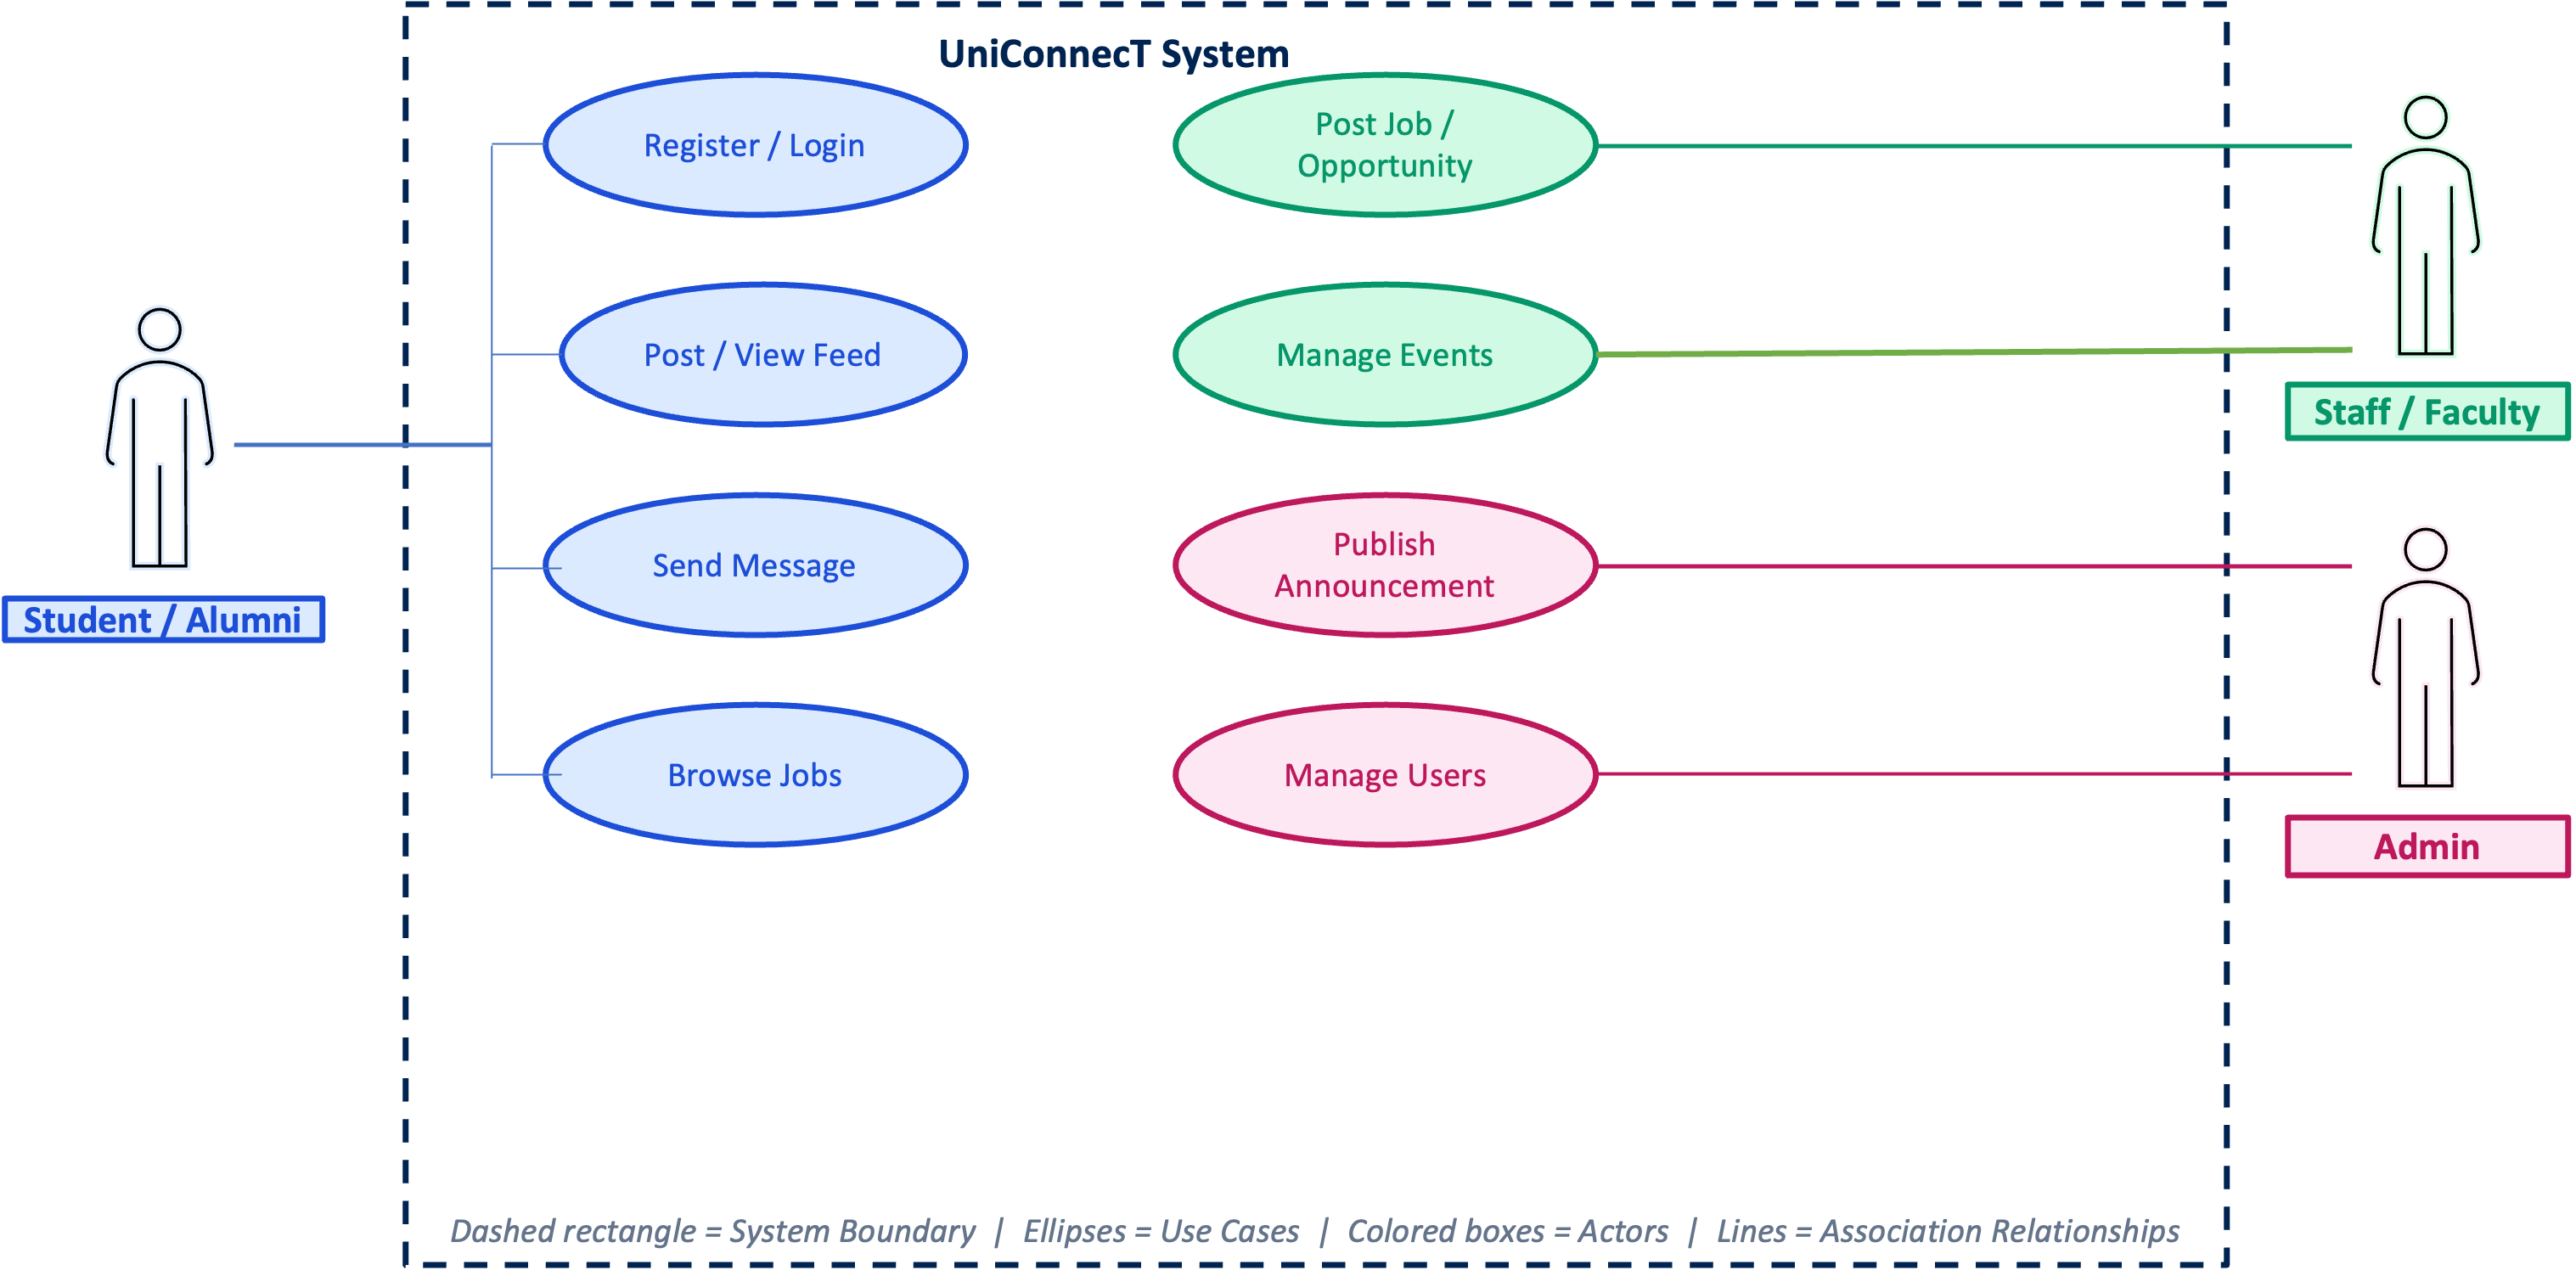
\includegraphics[width=0.92\textwidth, keepaspectratio]{diagrams/use_case_diagram.png}
    \caption{Use-case diagram for UniConnecT. Three actor groups ---
    Student/Alumni, Staff/Faculty, and Admin --- interact with core use cases
    including Register/Login, Post/View Feed, Send Message, Browse Jobs,
    Post Job/Opportunity, Manage Events, Publish Announcement, and Manage Users.
    Lines indicate association relationships between actors and the use cases
    they are permitted to invoke within the system boundary.}
    \label{fig:use_case}
\end{figure}

\begin{figure}[H]
    \centering
    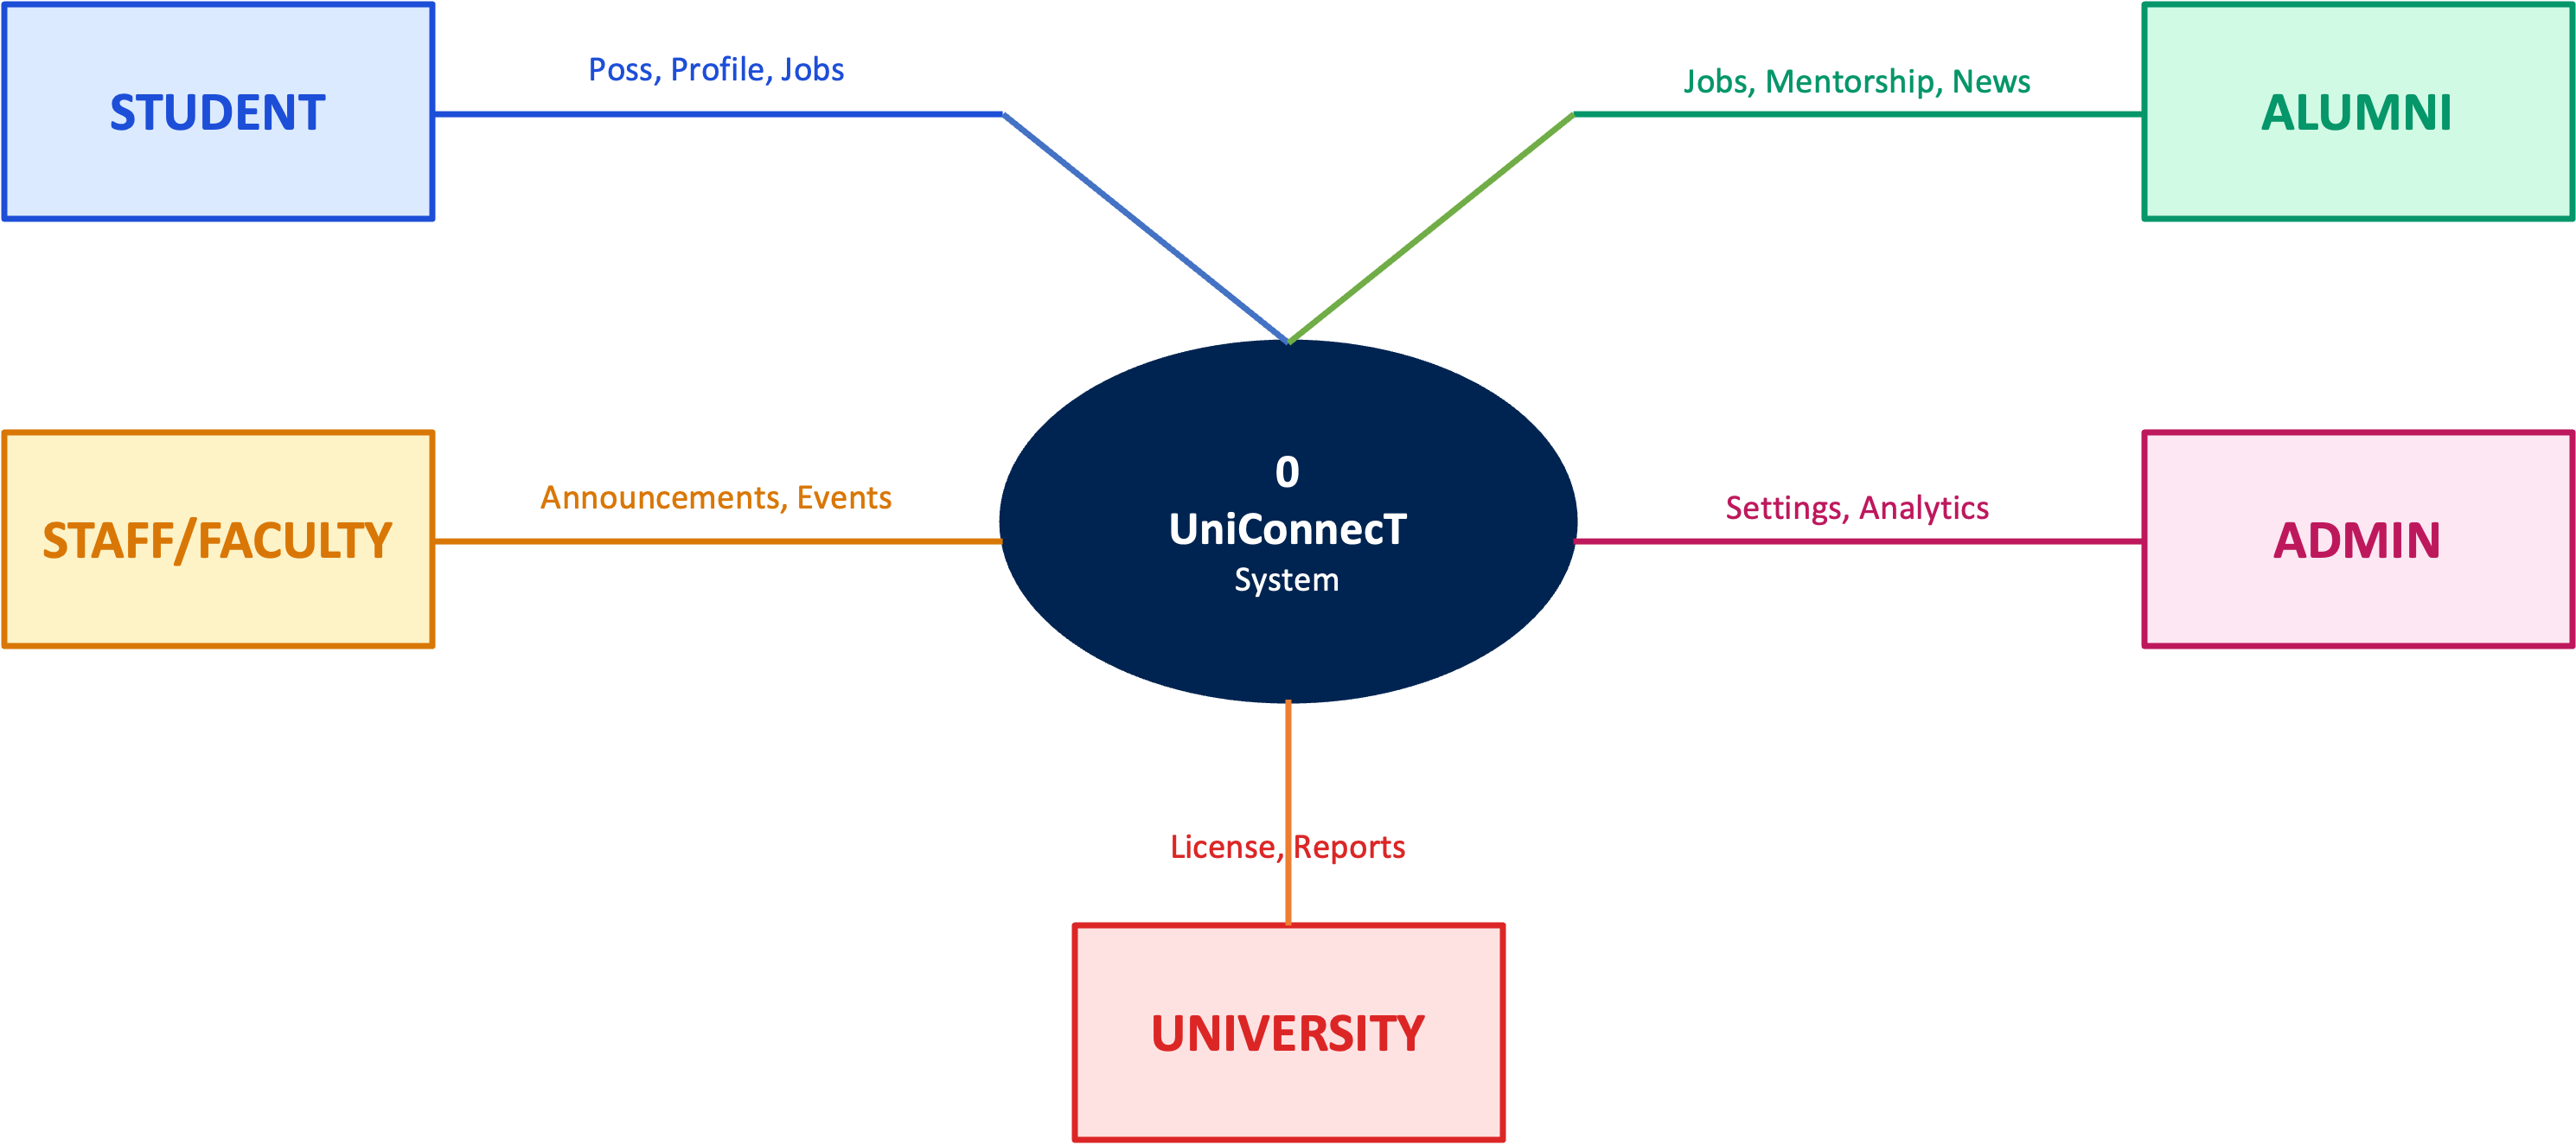
\includegraphics[width=0.92\textwidth, keepaspectratio]{diagrams/context_diagram.png}
    \caption{System context diagram (Level 0 DFD). UniConnecT occupies the central
    node. Five external entities interact with the system: Student (Posts, Profile,
    Jobs), Alumni (Jobs, Mentorship, News), Staff/Faculty (Announcements, Events),
    Admin (Settings, Analytics), and University (License, Reports). Data flows on
    each edge represent the primary information exchanged between each entity and
    the platform.}
    \label{fig:context}
\end{figure}
\clearpage
% ---------------------------------------------------------------
\section{Feasibility Analysis}
% ---------------------------------------------------------------

Feasibility analysis examines whether UniConnecT is viable from market, technical,
and financial perspectives within the two-year horizon of the project.

\subsection{Market Analysis}

\textbf{Total addressable market.}
Bangladesh has 54 approved private universities (UGC data, 2025) with a combined
active student enrolment exceeding 600,000. Each university operates at least one
administrative domain and runs independent communication channels. There is currently
no university-specific SaaS social platform serving this market.

\textbf{Serviceable addressable market.}
Of the 54 private universities, approximately 30 have active digital presences,
dedicated IT departments, and the budget infrastructure compatible with a SaaS
subscription model. The serviceable market is therefore $\approx30$ universities in
the first two years.

\textbf{Serviceable obtainable market (2-year target).}
A conservative penetration rate of 33\% of the serviceable market yields a two-year
target of 10 university deployments. At a per-university subscription of
\$500 per month, the obtainable annual recurring revenue at full Year~2 capacity is
\$60,000 USD.

\textbf{Pricing rationale.}
The subscription covers hosting (Azure App Service + Neon PostgreSQL + Redis), cloud
storage (Cloudflare R2), email delivery (Resend), and ongoing maintenance. At
\$500/month, the break-even unit cost per deployment is below \$200/month at 10+
active tenants, yielding a healthy gross margin above 60\%.

\begin{figure}[H]
    \centering
    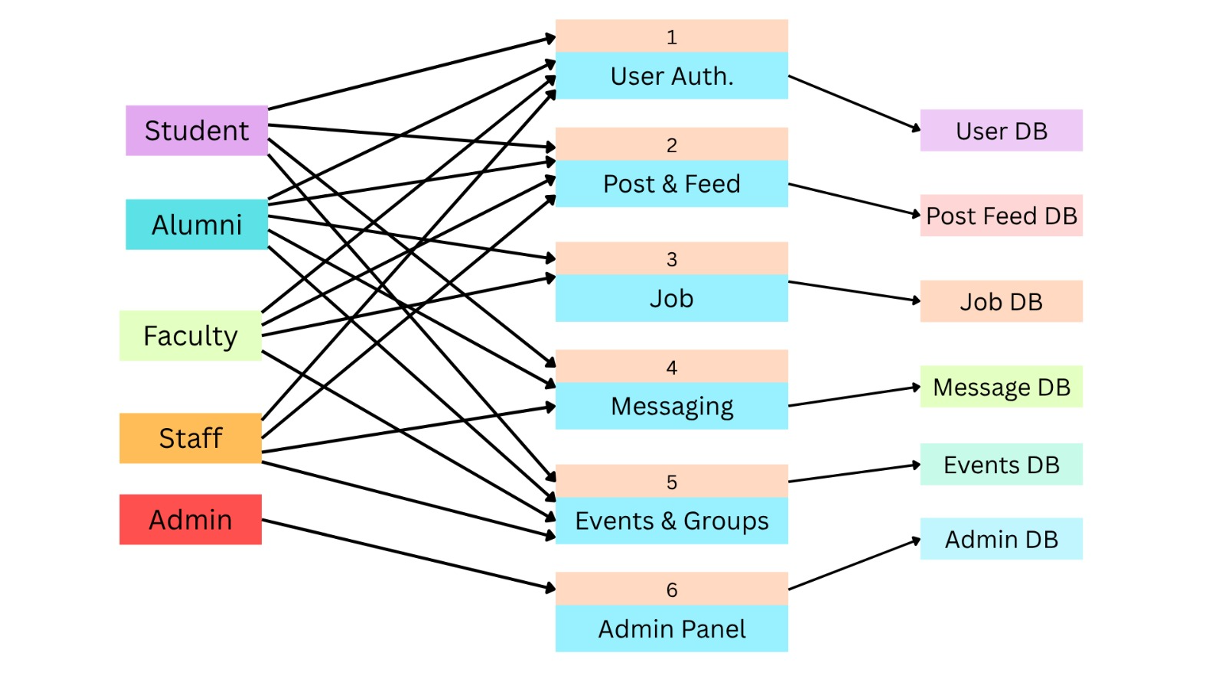
\includegraphics[width=0.92\textwidth, keepaspectratio]{diagrams/dfd.png}
    \caption{Data flow diagram (Level~1) for UniConnecT. Shows how data originates
    from five actor types (Student, Alumni, Faculty, Staff, Admin), flows through six
    processing modules (User Auth, Post \& Feed, Job, Messaging, Events \& Groups,
    Admin Panel), and is persisted in six data stores (User DB, Post Feed DB, Job DB,
    Message DB, Events DB, Admin DB). Arrows indicate the direction of data movement
    between actors, processes, and stores.}
    \label{fig:dfd}
\end{figure}

\begin{figure}[H]
    \centering
    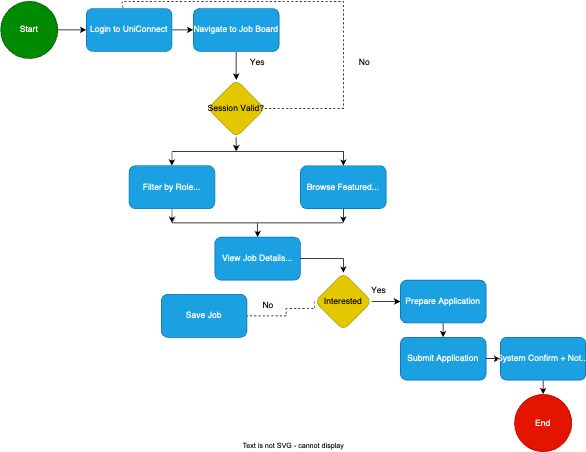
\includegraphics[width=0.92\textwidth, keepaspectratio]{diagrams/activity.png}
    \caption{Activity diagram illustrating a student's end-to-end job application
    journey on UniConnecT. The flow begins at Login, proceeds to the Job Board
    (gated by a Session Valid decision), allows the user to Filter by Role or
    Browse Featured listings, view job details, and then branches on interest:
    saving the job or preparing and submitting an application, which concludes
    with a system confirmation and notification.}
    \label{fig:activity}
\end{figure}

\subsection{Cash Flow and NPV Analysis}

The financial model below projects costs and revenues over a 24-month window
(July 2026 --- June 2028) using a discount rate of \textbf{10\% per annum}, which
approximates the opportunity cost of capital for an early-stage software project.

\textbf{Assumptions:}
\begin{itemize}
    \item Development team: 4 members × 6 months at \$2,000/month each = \$48,000
    total initial investment (Year~0, already incurred in development).
    \item Operating costs Year~1: hosting \$3,600 + marketing \$2,400 +
    maintenance support \$6,000 = \$12,000.
    \item Operating costs Year~2: hosting \$7,200 + marketing \$4,800 +
    maintenance support \$8,000 = \$20,000.
    \item Universities onboarded: 4 in Year~1, scaling to 12 by end of Year~2.
    \item Average subscription: \$500/month per university.
\end{itemize}

\begin{table}[H]
\centering
\renewcommand{\arraystretch}{1.3}
\begin{tabular}{p{5.5cm} r r r}
\toprule
\textbf{Item} & \textbf{Year 0} & \textbf{Year 1} & \textbf{Year 2} \\
              & \textbf{(\$USD)} & \textbf{(\$USD)} & \textbf{(\$USD)} \\
\midrule
\textit{Inflows} & & & \\
\quad Subscription revenue        & ---     & 24,000  & 72,000  \\
\midrule
\textit{Outflows} & & & \\
\quad Initial development cost    & (48,000) & ---    & ---     \\
\quad Operating costs             & ---      & (12,000) & (20,000) \\
\midrule
\textbf{Net cash flow}            & \textbf{(48,000)} & \textbf{12,000} & \textbf{52,000} \\
\midrule
Discount factor $(1.10)^{n}$      & 1.0000  & 1.1000  & 1.2100  \\
Present value of net cash flow    & (48,000.00) & 10,909.09 & 42,975.21 \\
\midrule
\textbf{Cumulative NPV}           & \textbf{(48,000.00)} & \textbf{(37,090.91)} & \textbf{+5,884.30} \\
\bottomrule
\end{tabular}
\caption{Two-year cash flow projection and NPV calculation (discount rate 10\%).}
\end{table}

\textbf{Net Present Value (NPV):}

\[
\text{NPV} = -48{,}000 + \frac{12{,}000}{(1.10)^{1}} + \frac{52{,}000}{(1.10)^{2}}
= -48{,}000 + 10{,}909.09 + 42{,}975.21 = \mathbf{\$5{,}884.30}
\]

Since NPV $> 0$, the project generates a positive return within the two-year window at
the assumed 10\% discount rate. Payback is achieved during Year~2 as cumulative
discounted cash flows cross break-even at approximately Month~21.

\textbf{Sensitivity note.} The NPV is sensitive to university acquisition rate.
Signing just 2 additional universities in Year~1 (6 total instead of 4) raises
Year~1 revenue by \$12,000 and improves NPV to approximately \$16,800 --- a 185\%
increase in project value, underscoring the leverage of early client acquisition.

% ---------------------------------------------------------------
\section{MoSCoW Model}
% ---------------------------------------------------------------

The MoSCoW model categorises all UniConnecT features by priority to guide
development sequencing. The model reflects the current state of the implemented
codebase and was validated against stakeholder requirements.

\begin{figure}[H]
    \centering
    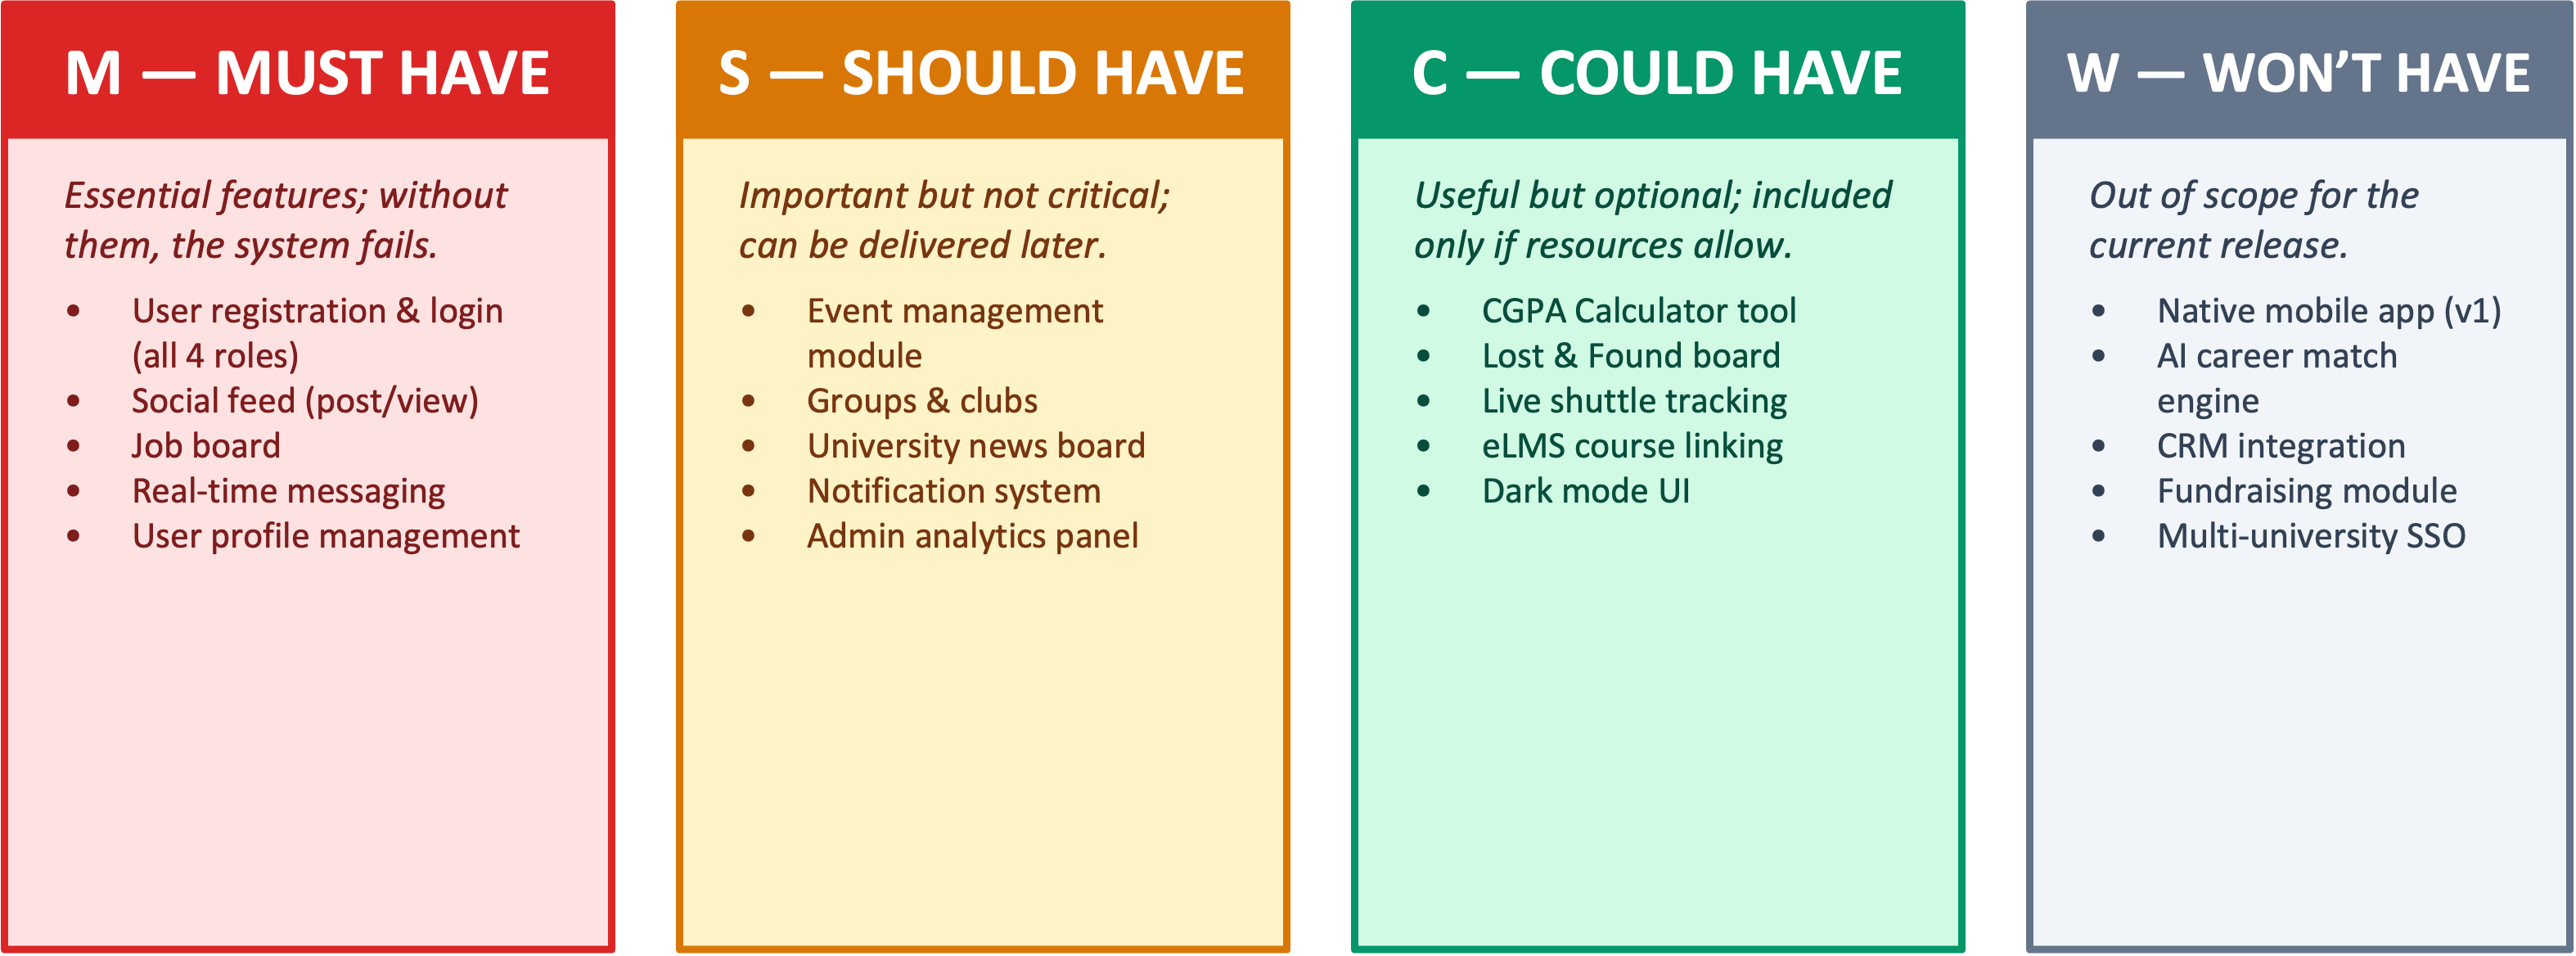
\includegraphics[width=0.88\textwidth, keepaspectratio]{diagrams/moscow.png}
    \caption{MoSCoW prioritisation matrix for UniConnecT. The four quadrants (Must
    Have, Should Have, Could Have, Won't Have) map each feature to its delivery
    commitment for the current release. Features in the Must Have quadrant were
    treated as hard scope; their absence would render the platform non-functional for
    the target university community.}
    \label{fig:moscow}
\end{figure}

\subsection{Must Have}

These features are non-negotiable and are fully implemented in the current release.
Without them, the platform cannot operate as a university social network.

\begin{itemize}
    \item \textbf{Invite-token registration with email OTP verification} --- ensures
    only verified university members can join.
    \item \textbf{JWT authentication with silent refresh} --- stateless, secure session
    management with 15-minute access tokens and 7-day refresh cookies.
    \item \textbf{Role-based access control} (student, alumni, faculty, admin, driver)
    --- each role sees and can perform only what the university authorises.
    \item \textbf{Social feed} (create, react, comment, share posts) --- the core
    engagement surface of the platform.
    \item \textbf{Real-time messaging} (direct, group, mentorship threads) ---
    Socket.io powered, scaled via Redis pub/sub.
    \item \textbf{User profiles with experience, education, and skills} --- foundation
    of professional identity on the platform.
    \item \textbf{University-scoped data isolation} --- multi-tenant architecture;
    every DB row carries \texttt{university\_id}; no cross-university data leakage.
    \item \textbf{Admin panel} (user management, invitations, content reports) ---
    universities cannot operate the platform without institutional governance.
    \item \textbf{Notifications} (in-app + Web Push) --- users must be informed of
    relevant activity in real time.
\end{itemize}

\subsection{Should Have}

These features significantly enhance the value proposition and are implemented in the
current release, though the platform would still function at a basic level without them.

\begin{itemize}
    \item \textbf{Job and internship board} --- alumni-posted opportunities scoped to
    the university; application tracking for students.
    \item \textbf{Events management} with RSVP --- creation, browsing, and attendance
    tracking for campus events.
    \item \textbf{Groups and clubs} --- private/public groups with member roles,
    resources, study sessions, pinned posts, and group rules.
    \item \textbf{Mentorship module} --- request/accept flow, session logging, points
    economy, alumni capacity enforcement, gift card redemption.
    \item \textbf{Full-text search} --- Postgres generated \texttt{search\_vector}
    columns across profiles, posts, jobs, events, and groups.
    \item \textbf{University news feed} with content-sync engine --- auto-import
    from WordPress/external CMS with admin review workflow.
    \item \textbf{Connections (LinkedIn-style)} --- bidirectional connection graph
    replacing the old follow model.
    \item \textbf{Profile analytics} (7/30/90-day view counts, viewer list) ---
    professional insight into profile reach.
\end{itemize}

\subsection{Could Have}

These features add value but were treated as stretch goals. A subset is implemented;
the remainder is scoped for future iterations.

\begin{itemize}
    \item \textbf{Draft posts across content types} --- save-and-resume authoring
    for posts, jobs, events, and news articles. \textit{(Implemented.)}
    \item \textbf{Explore page} with trending tags and suggested users.
    \textit{(Implemented.)}
    \item \textbf{Resume export} from profile data to a downloadable PDF.
    \textit{(Implemented.)}
    \item \textbf{Dark/light theme toggle} with user preference persistence.
    \textit{(Implemented.)}
    \item \textbf{Presence indicators} --- real-time online/offline status with
    privacy tier controls. \textit{(Implemented.)}
    \item \textbf{Group digest email} (weekly summary of group activity via Bull cron).
    \textit{(Implemented.)}
    \item \textbf{Mobile-responsive design} --- full Tailwind CSS responsive layout.
    \textit{(Implemented.)}
    \item \textbf{Skyvern browser-automation fallback} for content sync when WordPress
    REST API is unavailable. \textit{(Implemented.)}
\end{itemize}

\subsection{Won't Have (This Release)}

These features were explicitly deferred to avoid scope creep. They remain on the
long-term product roadmap.

\begin{itemize}
    \item \textbf{Native mobile applications} (iOS / Android) --- the current release
    is a progressive web app only; native apps require a separate development cycle.
    \item \textbf{Video calling or live streaming} --- real-time video would require
    WebRTC infrastructure and per-stream bandwidth cost modelling beyond current scope.
    \item \textbf{AI-powered feed curation} --- machine learning recommendations
    require training data volume only achievable after several months of live usage.
    \item \textbf{Cross-university alumni network} --- multi-university interaction
    conflicts with the institution-bound privacy model and requires a governance
    redesign.
    \item \textbf{Integrated payment gateway} --- monetised mentorship sessions and
    paid events are deferred pending legal and financial compliance review.
    \item \textbf{User self-deletion} --- account deletion is admin-mediated
    (request-with-reason workflow) to preserve audit integrity and data retention
    compliance.
\end{itemize}
\clearpage
% ---------------------------------------------------------------
\section{Kano Model}
% ---------------------------------------------------------------

The Kano model classifies UniConnecT features by the nature of their relationship
to user satisfaction. It distinguishes between features that users expect as
table-stakes (Basic), features where more is always better (Performance), and
features that unexpectedly delight users when present (Excitement).

\begin{figure}[H]
    \centering
    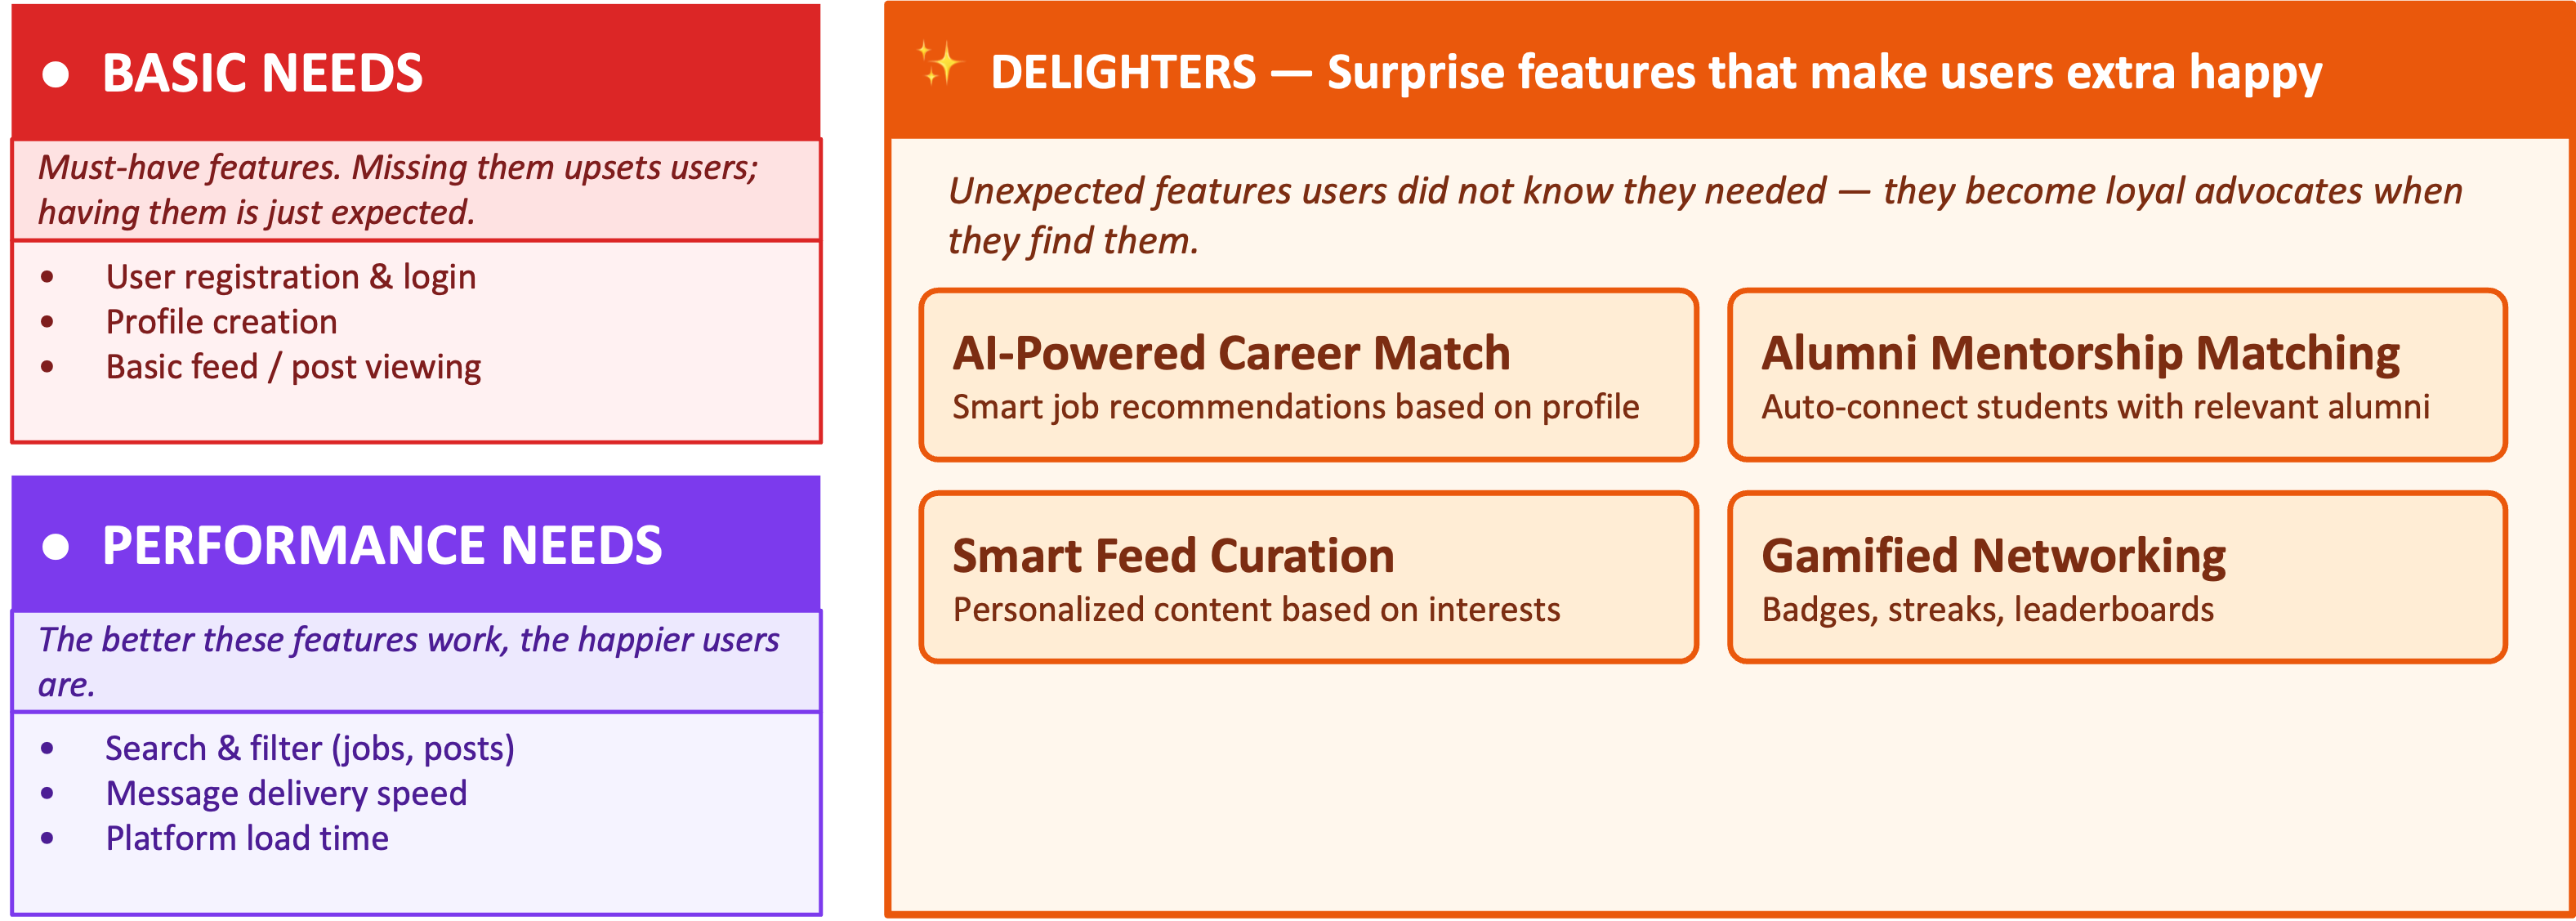
\includegraphics[width=0.88\textwidth, keepaspectratio]{diagrams/kano.png}
    \caption{Kano model overview for UniConnecT, organised as three feature categories.
    \textit{Basic Needs} (must-be quality): user registration/login, profile creation,
    and basic feed viewing --- their absence causes immediate dissatisfaction.
    \textit{Performance Needs}: search \& filter, message delivery speed, and platform
    load time --- satisfaction scales linearly with quality.
    \textit{Delighters}: AI-powered career match, alumni mentorship matching, smart
    feed curation, and gamified networking --- unexpected features that create strong
    positive reactions when discovered.}
    \label{fig:kano}
\end{figure}

\subsection{Basic (Must-Be) Quality Features}

These features are taken for granted when present; their absence causes immediate
dissatisfaction and platform rejection. They are threshold requirements, not
differentiators.

\begin{itemize}
    \item \textbf{Secure login and session management} --- users expect authentication
    to simply work. Any failure here (token leaks, silent logouts) destroys trust
    immediately.
    \item \textbf{Fast page loads and responsive UI} --- users expect sub-2-second
    render times on any device. Slowness is a hygiene failure.
    \item \textbf{Reliable notification delivery} --- missing a job offer notification
    or mentorship acceptance is an unacceptable failure, not a missing feature.
    \item \textbf{Data privacy and access isolation} --- users expect their content to
    be visible only to their university community. A cross-tenant data leak would
    terminate the product.
    \item \textbf{Mobile-readable layout} --- the majority of students access platforms
    on mobile. A desktop-only layout would exclude a large fraction of the user base.
    \item \textbf{Profile completeness} --- name, photo, role, and department are
    expected to be present and editable. An incomplete identity layer undermines trust
    in every other interaction.
\end{itemize}

\subsection{Performance Quality Features}

These features directly scale satisfaction with the quality of their implementation.
The better the feature works, the happier the user; degraded performance causes
proportional dissatisfaction.

\begin{itemize}
    \item \textbf{Feed relevance and ranking} --- a chronological feed is baseline;
    the HN-style \texttt{hot\_score} ranking algorithm and ``Top'' feed sort increase
    satisfaction linearly as relevance improves.
    \item \textbf{Search accuracy and speed} --- the quality of full-text search
    (Postgres GIN-indexed \texttt{search\_vector} with tsvector weighting A/B/C) maps
    directly to how quickly users find peers, jobs, or content.
    \item \textbf{Mentorship match quality} --- the usefulness of the mentorship
    module scales with how well students can discover the right mentor by field,
    seniority, and availability.
    \item \textbf{Job board coverage} --- the more alumni post opportunities, the more
    valuable the board. Coverage is the primary performance dimension of this feature.
    \item \textbf{Message delivery latency} --- real-time chat satisfaction correlates
    directly with message round-trip latency. Sub-100ms delivery (Redis pub/sub, local
    Socket.io) feels instant; anything above 500ms feels broken.
    \item \textbf{Content sync freshness} --- the news module's value scales with how
    recently the WordPress importer has run. Stale news is worse than no news.
\end{itemize}

\subsection{Excitement (Delighter) Features}

These features are not anticipated by users. When discovered, they generate strong
positive reactions and become key advocates of the platform. Their absence causes no
dissatisfaction.

\begin{itemize}
    \item \textbf{Points-based mentorship economy with gift card redemption} --- alumni
    earn redeemable points for mentorship sessions. No university platform offers this;
    users who discover it are strongly motivated to participate.
    \item \textbf{Live shuttle GPS tracking} --- students discovering real-time bus
    location on a campus social app is wholly unexpected and immediately useful.
    \item \textbf{Resume PDF export from profile} --- turning the platform profile
    into a downloadable resume surprises users accustomed to maintaining separate CVs.
    \item \textbf{Skyvern-powered news auto-import} --- administrators discover that
    the platform automatically harvests university news from external CMS sources via
    browser automation when the standard API is unavailable.
    \item \textbf{Profile view analytics} (7/30/90-day viewer list) --- users do not
    expect to see who has viewed their profile. Discovering this feature creates
    immediate engagement loops and motivates profile completion.
    \item \textbf{Presigned S3 upload flow} --- file attachments upload directly from
    the browser to cloud storage with zero server-side byte handling. Users experience
    this as surprising speed; developers appreciate the architectural elegance.
\end{itemize}
\clearpage
% ---------------------------------------------------------------
\section{Functional Requirements}
% ---------------------------------------------------------------

The functional requirements define the specific behaviors and capabilities the
UniConnecT system shall provide. Each requirement is labeled with a unique identifier
for traceability.

\subsection{Authentication and Account Management}

\begin{enumerate}[label=\textbf{FR-\arabic*:}, leftmargin=*, align=left]

    \item The system shall allow new users to register using a valid university
    invitation token, providing their full name, email address, and a chosen password.

    \item The system shall send a one-time password (OTP) to the user's registered
    email address upon registration, which must be confirmed to activate the account.

    \item The system shall allow registered users to log in with their email and
    password and log out securely from any session.

    \item The system shall support a password recovery flow that allows users to
    request a reset link via their registered university email address.

    \item The system shall validate all user input during registration and login,
    displaying clear inline error messages for missing or invalid fields.

\end{enumerate}

\subsection{Social Feed and Content Management}

\begin{enumerate}[label=\textbf{FR-\arabic*:}, leftmargin=*, align=left]
\setcounter{enumi}{5}

    \item The system shall display a personalized social feed upon login, showing
    posts, reactions, and activity from the user's university community, sortable
    by ``Recent'' and ``Top'' (engagement-ranked) modes.

    \item The system shall allow users to create, edit, delete, and save draft posts
    on the social feed, with support for text content, images, and links.

    \item The system shall allow users to react to and comment on any post in the
    feed, with real-time count updates.

\end{enumerate}

\subsection{Profiles, Connections, and Search}

\begin{enumerate}[label=\textbf{FR-\arabic*:}, leftmargin=*, align=left]
\setcounter{enumi}{8}

    \item The system shall allow users to view and edit their own profile, including
    profile photo, bio, work experience entries, education history, skills, and
    featured items (maximum five).

    \item The system shall track profile views and provide each profile owner with
    an analytics view showing visitor counts over the past 7, 30, and 90 days,
    along with a list of recent viewers.

    \item The system shall allow users to send, accept, decline, and withdraw
    connection requests. Accepted connections form a persistent, bidirectional
    professional network visible on each user's profile.

    \item The system shall display connection suggestions to users based on mutual
    connections and shared university affiliation.

    \item The system shall provide a unified full-text search interface through which
    users can search for people, posts, jobs, events, groups, and news by keyword,
    with filterable result tabs per content type.

\end{enumerate}

\subsection{Jobs, Events, and Groups}

\begin{enumerate}[label=\textbf{FR-\arabic*:}, leftmargin=*, align=left]
\setcounter{enumi}{13}

    \item The system shall allow alumni and faculty to post job and internship
    listings specifying role title, description, requirements, and application
    deadline.

    \item The system shall display job listings in a filterable, sortable list view,
    with a detail page for each listing.

    \item The system shall allow users to create and browse campus events, with RSVP
    functionality and a detail view showing date, location, description, and confirmed
    attendee count.

    \item The system shall allow users to create, join, and leave groups (clubs,
    departments, study circles), with public and private group types. Private groups
    require a join request approved by a group administrator.

    \item The system shall allow group administrators to manage member roles
    (admin, moderator, member), pin posts, post group rules, share file resources
    with view tracking, and schedule study sessions with RSVP.

\end{enumerate}

\subsection{Messaging, Notifications, and Mentorship}

\begin{enumerate}[label=\textbf{FR-\arabic*:}, leftmargin=*, align=left]
\setcounter{enumi}{18}

    \item The system shall provide real-time direct messaging between any two
    connected users, and group messaging within shared conversation threads.

    \item The system shall automatically create a dedicated conversation thread
    for each accepted mentorship request, linking the student and the alumni
    mentor within the messaging module.

    \item The system shall deliver real-time in-app notifications for events including
    new connection requests, accepted connections, new messages, post reactions,
    mentions, event updates, and mentorship activity.

    \item The system shall allow students to send mentorship requests to alumni,
    specifying their goals and area of guidance sought. Alumni may accept or decline
    requests subject to their configured maximum mentee capacity.

\end{enumerate}

\subsection{Campus Utilities, Administration, and Settings}

\begin{enumerate}[label=\textbf{FR-\arabic*:}, leftmargin=*, align=left]
\setcounter{enumi}{22}

    \item The system shall allow users to browse and read official university news
    and announcements published by faculty or administrators, with a detail page
    per article.

    \item The system shall provide a lost-and-found module where users can post
    reports of lost or found campus items, including a description, location, and
    optional photo.

    \item The system shall display campus shuttle route schedules and real-time
    shuttle location, updated continuously from driver GPS broadcasts.

    \item The system shall allow drivers (driver role exclusively) to broadcast
    their GPS location via a dedicated interface, which is reflected live on the
    student-facing shuttle tracker.

    \item The system shall provide an administrator panel through which admins can
    manage user accounts, assign and change roles, create and revoke invitation
    tokens (including bulk invitations), resolve content reports, and configure
    university-wide settings.

    \item The system shall aggregate all of a user's unpublished drafts --- across
    posts, job listings, news articles, and events --- into a single drafts view
    accessible only by the author.

    \item The system shall allow users to configure notification preferences,
    privacy settings (profile visibility, presence visibility, message
    accessibility), and application appearance (light or dark theme) from a
    dedicated settings hub.

\end{enumerate}

\clearpage
% ---------------------------------------------------------------
\section{Non-Functional Requirements}
% ---------------------------------------------------------------

Non-functional requirements specify the quality attributes and operational constraints
the UniConnecT design shall satisfy.

\subsection{Usability, Performance, and Responsiveness}

\begin{enumerate}[label=\textbf{NFR-\arabic*:}, leftmargin=*, align=left]

    \item \textbf{Usability:} The interface shall be intuitive and learnable, enabling
    a new student user to complete primary tasks --- registration, OTP verification,
    profile setup, browsing the feed, and sending a connection request --- without
    external documentation or guidance.

    \item \textbf{Consistency:} All pages shall adhere to the UniConnecT design system,
    maintaining a consistent color palette, typography (font weight restricted to 400
    and 500), spacing scale, border style (0.5px structural borders), and component
    visual language throughout. No hardcoded color values shall appear outside the
    defined token set.

    \item \textbf{Responsiveness:} The interface shall render correctly and remain fully
    usable across three primary breakpoints: mobile (360px--767px), tablet
    (768px--1023px), and desktop (1024px and above). Navigation shall collapse to a
    bottom tab bar on mobile; multi-column layouts shall reflow to single-column views.

    \item \textbf{Performance (Perceived):} The feed, dashboard, profile, and listing
    pages shall use skeleton loading states during data load, ensuring the interface
    appears immediately responsive and never presents a blank screen to the user.

    \item \textbf{Accessibility:} All text-on-background color combinations in both
    the dark and light themes shall meet a minimum 4.5:1 contrast ratio (WCAG 2.1
    Level AA). All interactive elements shall carry visible focus states. All form
    inputs shall have descriptive labels; icon-only controls shall include tooltips.

    \item \textbf{Feedback and Error Handling:} The design shall include explicit
    visual states for every user action: button hover, loading, success, and error.
    Inline validation errors shall appear adjacent to the failing field. All list
    and feed views shall have a designed empty state rather than a blank area.

\end{enumerate}

\subsection{Access Control, Theming, and Maintainability}

\begin{enumerate}[label=\textbf{NFR-\arabic*:}, leftmargin=*, align=left]
\setcounter{enumi}{6}

    \item \textbf{Role-Based Interface Separation:} The design shall strictly enforce
    role-aware navigation and page access. The admin panel shall not surface in
    navigation for non-admin roles. The driver GPS broadcast view shall be accessible
    only to driver-role users. Students, alumni, and faculty shall each see a
    navigation set scoped to their role's permitted features.

    \item \textbf{Dual-Theme Support:} The design system shall define both a
    \textit{Warm Futuristic Dark} default theme (navy surfaces, UIU orange accent,
    indigo interactive states) and a \textit{Warm Neutral Light} theme. All
    components shall be designed to render correctly in both themes without
    design-level modifications per page.

    \item \textbf{Modifiability:} The Figma design system shall use shared component
    libraries (atoms and molecules) so that any design system change --- color,
    typography, spacing, border radius --- propagates consistently across all pages
    without requiring individual page edits.

    \item \textbf{Readability:} Body text shall be set at a minimum of 14px with
    adequate line-height. Section headings shall establish hierarchy through size
    and weight differences alone, not color. All UI labels and button text shall use
    sentence case; no ALL CAPS labels shall appear anywhere in the interface.

\end{enumerate}

\clearpage
% ---------------------------------------------------------------
\section{Pages / Modules}
% ---------------------------------------------------------------

The following pages and modules constitute the UniConnecT Figma prototype. Each entry
represents a distinct screen or logical section of the planned application.

\subsection{Public and Authentication Pages}

\begin{enumerate}
    \item \textbf{Landing Page} --- The public entry point of UniConnecT, presenting
    the platform's value proposition with a hero section and calls to action
    (``Join Your University Network'', ``Log In'').

    \item \textbf{Registration Page} --- An invitation-token-gated sign-up form
    collecting the user's full name, email address, and password.

    \item \textbf{OTP Verification Page} --- A code-entry screen for confirming the
    user's email address using the one-time password sent upon registration.

    \item \textbf{Login Page} --- A secure sign-in form for registered users with
    inline validation and a ``Forgot Password'' link.

    \item \textbf{Forgot Password / Reset Password Page} --- A two-step recovery
    flow: the user submits their email, then follows a link to set a new password.
\end{enumerate}

\subsection{Core Social and Professional Pages}

\begin{enumerate}
\setcounter{enumi}{5}
    \item \textbf{Social Feed (Home / Dashboard)} --- The primary authenticated
    screen displaying a ranked, scrollable feed of community posts, with ``Recent''
    and ``Top'' sort tabs, a left-side profile summary panel, and a right-side
    discovery sidebar.

    \item \textbf{Post Detail Page} --- A full-page view of a single post showing
    the complete content, all reactions, and a threaded comment section.

    \item \textbf{Profile Page} --- Displays a user's public profile: cover photo,
    avatar, bio, experience, education, skills, featured items, recent activity,
    and profile analytics. Includes an edit flow for the profile owner.

    \item \textbf{Connections / My Network Page} --- Shows the user's accepted
    connections, incoming pending requests, sent requests, and a ``People You May
    Know'' suggestions section.

    \item \textbf{Explore Page} --- A discovery screen for finding new community
    members, trending content, and activity outside the user's immediate connection
    network.

    \item \textbf{Search Results Page} --- A unified results screen with filterable
    tabs for People, Posts, Jobs, Events, Groups, and News.

    \item \textbf{Jobs Page} --- A filterable, sortable listing of job and internship
    postings within the university network, with a detail page per listing and a
    posting form for eligible users.

    \item \textbf{Events Page} --- A listing of upcoming campus events with RSVP
    functionality and a full detail view per event.

    \item \textbf{Groups Page} --- A directory of university groups and clubs, with
    a detail view per group showing the group feed, members list, file resources,
    scheduled study sessions, pinned posts, and group rules.

    \item \textbf{Messages Page} --- A real-time messaging interface with a
    conversation list sidebar and an active chat panel, supporting direct and
    group conversations as well as dedicated mentorship threads.

    \item \textbf{Notifications Page} --- A chronological list of all in-app
    notifications for the logged-in user, covering connections, messages, reactions,
    mentions, and mentorship activity.

    \item \textbf{News Page} --- A listing of official university news and
    announcements, with a detail view per article including title, body, and
    publication date.

    \item \textbf{Mentorship Page} --- A module where students browse alumni mentor
    profiles and submit mentorship requests, and where alumni manage their active
    mentees, session records, and mentee capacity.
\end{enumerate}

\subsection{Campus Utility Pages}

\begin{enumerate}
\setcounter{enumi}{18}
    \item \textbf{Lost \& Found Page} --- A campus utility module for posting and
    browsing reports of lost or found items, with descriptions, last-known location,
    and optional photo.

    \item \textbf{Shuttle Tracker Page} --- Displays campus shuttle route schedules
    and a live shuttle position map updated from driver GPS broadcasts.

    \item \textbf{Driver GPS Broadcast View} --- A minimal, role-restricted interface
    for transport drivers to broadcast their current GPS location to the platform.
\end{enumerate}

\subsection{Settings and Administration Pages}

\begin{enumerate}
\setcounter{enumi}{21}
    \item \textbf{Drafts Page} --- A personal page aggregating all of the user's
    unpublished drafts across posts, job listings, news articles, and events.

    \item \textbf{Settings Page} --- A multi-section hub covering appearance (light
    / dark theme), account management (deactivation, username), notification
    preferences, and privacy controls (profile, presence, and message visibility).

    \item \textbf{Admin Panel} --- A role-restricted management interface for
    administrators covering user management, role assignment, invitation management
    (individual and bulk), content report resolution, platform statistics, and
    university configuration.
\end{enumerate}

% ---------------------------------------------------------------
\section{Tools and Technologies}
% ---------------------------------------------------------------

This section covers the design and prototyping tools used for UniConnecT. It describes
the design process only.

\subsection{Design and Prototyping Tools}

\begin{itemize}
    \item \textbf{Figma} --- Primary tool for all UI/UX work: wireframing,
    high-fidelity mockups, interactive prototyping, and the shared component design
    system. All 24 pages and user flows are designed within Figma.

    \item \textbf{Figma Plugins:}
        \begin{itemize}
            \item \textit{Iconify} --- Used to source and insert scalable vector icons
            (Phosphor Icons and Heroicons sets) directly into Figma frames.
            \item \textit{Unsplash} --- Used to insert high-quality placeholder
            photography for profile avatars, event covers, and news thumbnails
            within mockups.
            \item \textit{A11y --- Color Contrast Checker} --- Used to verify that
            all text and UI element color pairings meet WCAG 2.1 Level AA contrast
            requirements across both dark and light themes.
        \end{itemize}

    \item \textbf{FigJam} --- Used to create the navigation flow diagram and module
    architecture diagram, leveraging FigJam's drag-and-drop connector tools and
    sticky-note layout for clear, readable system diagrams.
\end{itemize}

\subsection{Supporting and Auxiliary Tools}

\begin{itemize}
    \item \textbf{Canva} --- Used for supplementary graphics including the project
    cover slide, presentation visuals, and promotional design assets.

    \item \textbf{Google Fonts} --- Typography selections (Inter for UI labels and
    body text) sourced from Google Fonts and applied within the Figma design system.

    \item \textbf{Coolors} --- Used to explore and finalize the UniConnecT color
    palette for both the Warm Futuristic Dark theme (navy, UIU orange, indigo) and
    the Warm Neutral Light theme.
\end{itemize}
\clearpage
% ---------------------------------------------------------------
\section{System Design / Wireframe}
% ---------------------------------------------------------------

All visuals in this section are taken from the Figma design prototype. The figures
below present wireframes and UI sketches for the major pages of UniConnecT, along
with a navigation flow diagram and module architecture diagram.

\subsection{Authentication and Public Pages}

% --- Landing Page ---
\begin{figure}[H]
    \centering
    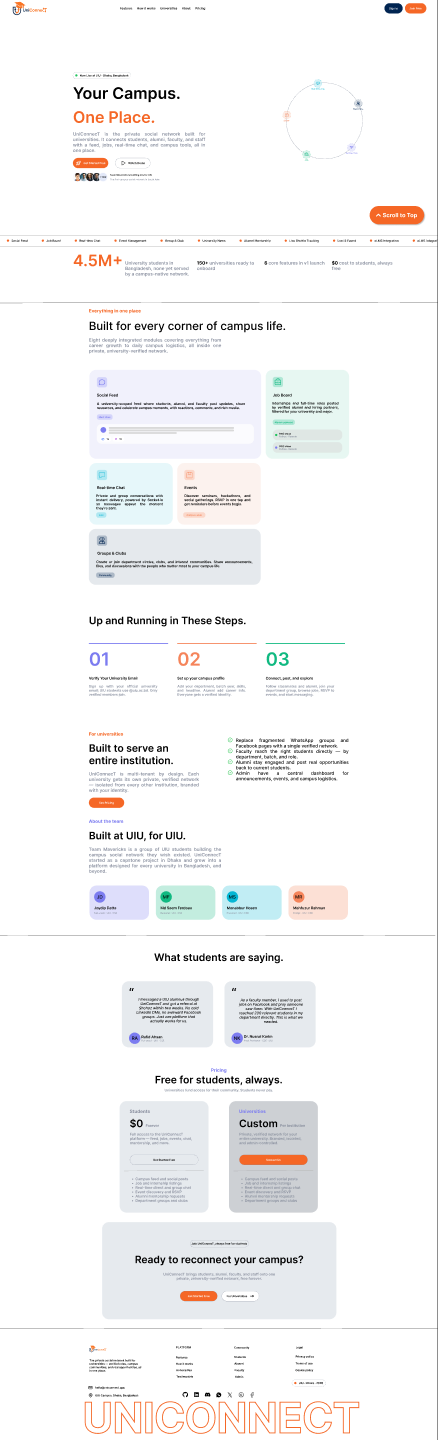
\includegraphics[width=0.85\textwidth, height=0.68\textheight, keepaspectratio]{figma_landing_page.png}
    \caption{Figma Wireframe --- Landing Page. The public entry screen with a hero
    section presenting UniConnecT's value proposition, a top navigation bar, and
    calls to action for new and returning users.}
    \label{fig:landing}
\end{figure}

% --- Login Page ---
\begin{figure}[H]
    \centering
    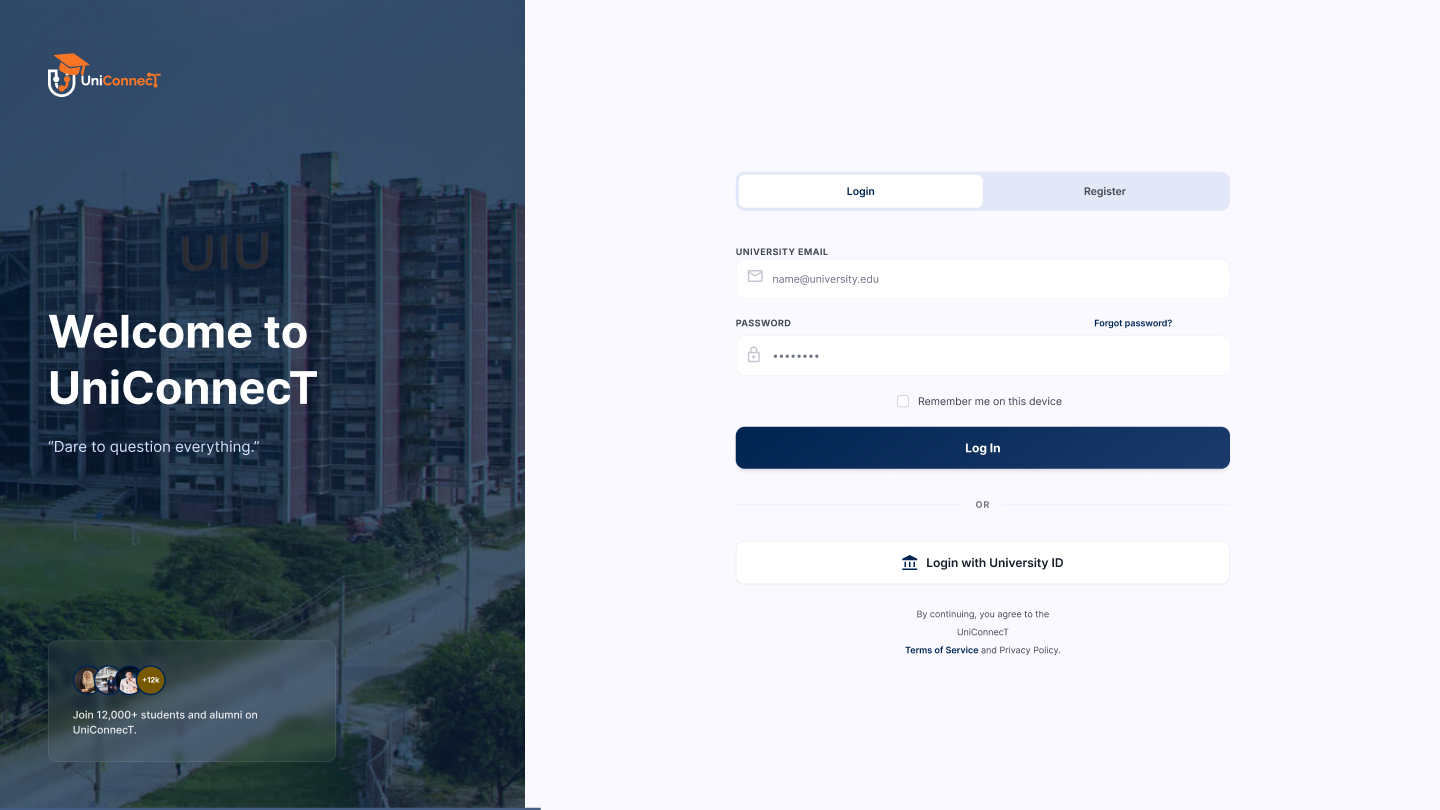
\includegraphics[width=0.85\textwidth, height=0.68\textheight, keepaspectratio]{figma_login_wireframe.png}
    \caption{Figma Wireframe --- Login Page. Email and password input form with inline
    validation states, a ``Forgot Password'' link, and the university domain context
    displayed in the header.}
    \label{fig:login}
\end{figure}

% --- Registration + OTP ---
\begin{figure}[H]
    \centering
    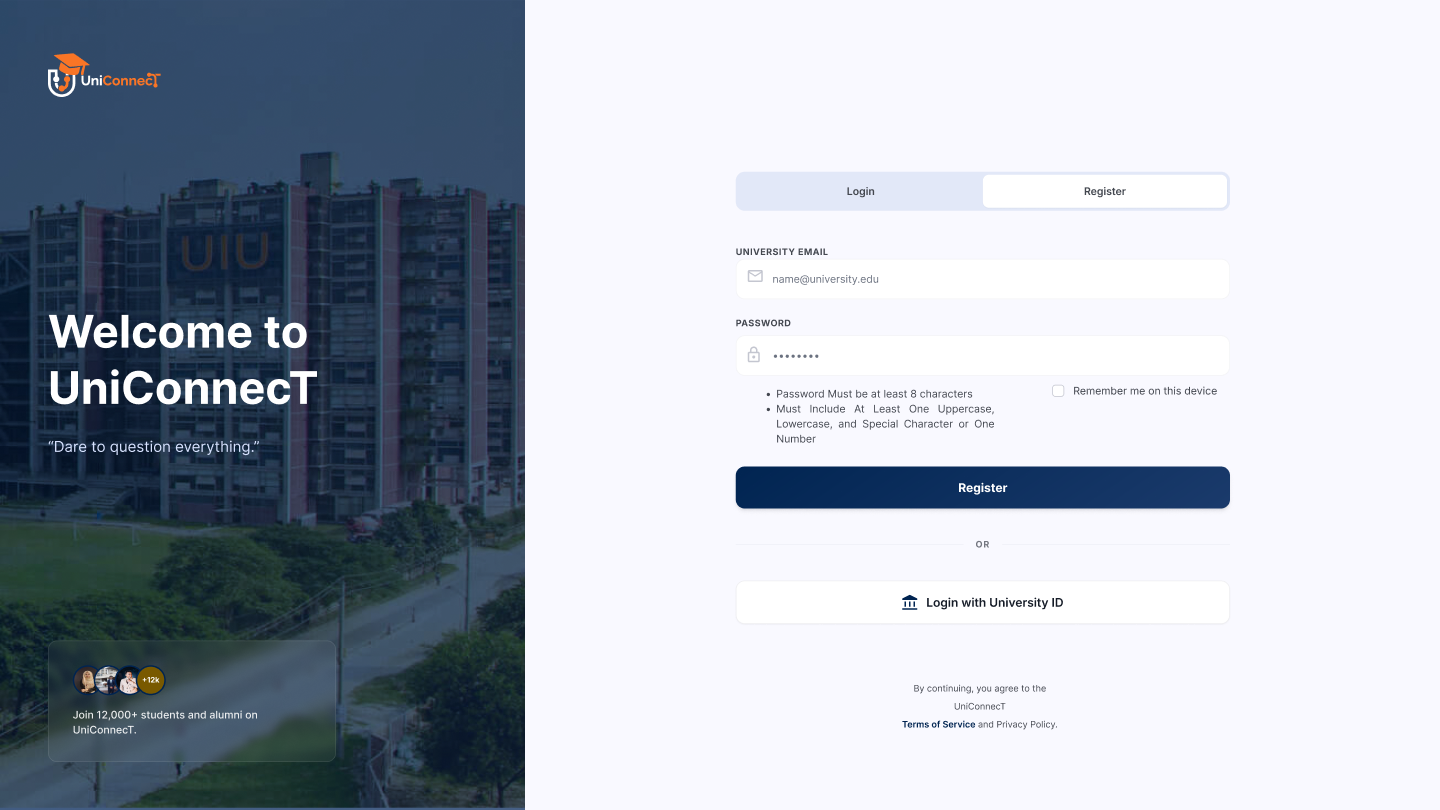
\includegraphics[width=0.85\textwidth, height=0.68\textheight, keepaspectratio]{figma_register_wireframe.png}
    \caption{Figma Wireframe --- Registration Page. Invitation-token-gated sign-up
    form collecting name, email, and password, followed by the OTP email verification
    step.}
    \label{fig:register}
\end{figure}

\subsection{Core Social and Professional Wireframes}

% --- Social Feed / Dashboard ---
\begin{figure}[H]
    \centering
    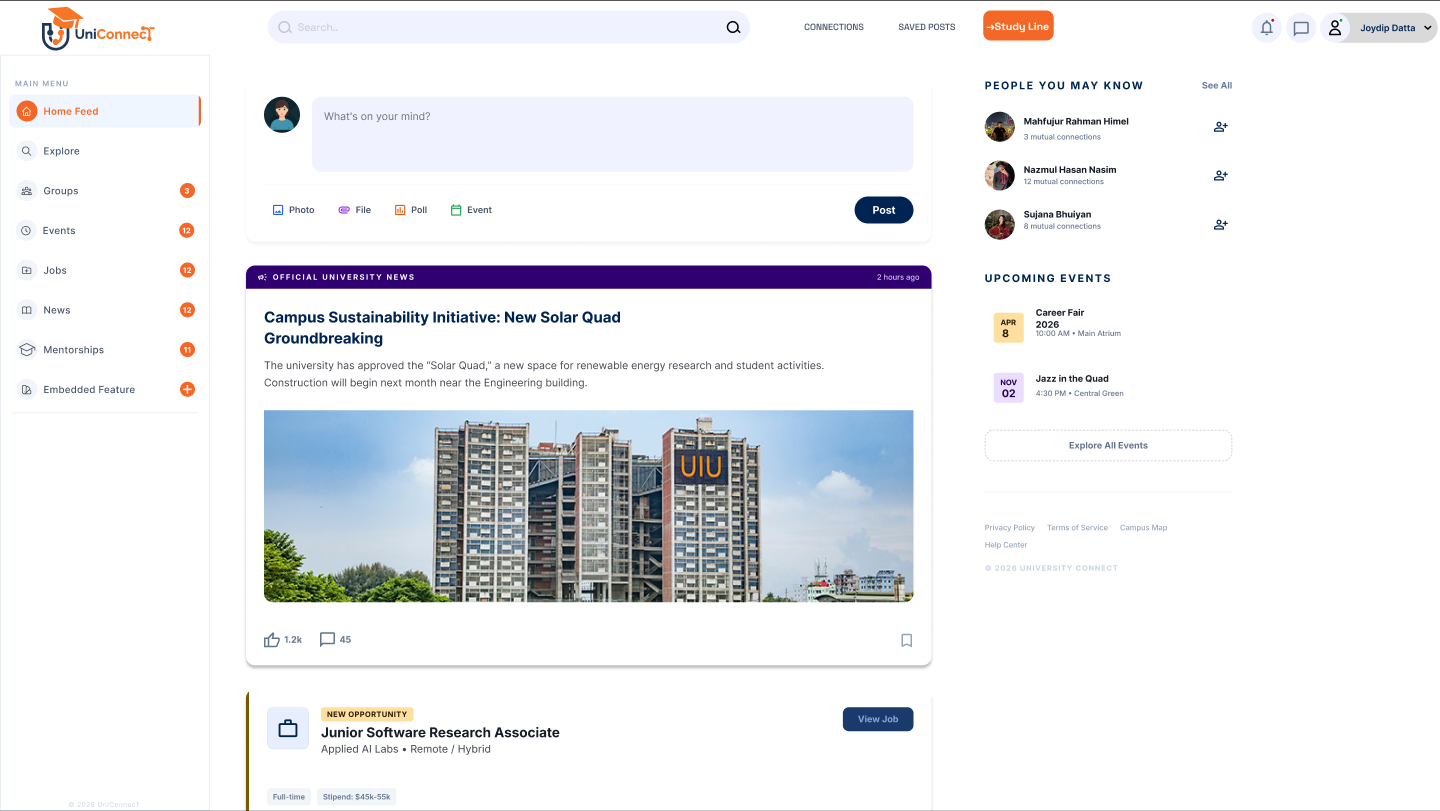
\includegraphics[width=0.85\textwidth, height=0.68\textheight, keepaspectratio]{figma_feed_dashboard.png}
    \caption{Figma Wireframe --- Social Feed (Dashboard). The main authenticated
    screen: ranked post feed in the centre, a profile summary panel on the left, and
    a discovery/suggestions sidebar on the right. ``Recent'' and ``Top'' feed tabs
    are shown.}
    \label{fig:feed}
\end{figure}

% --- Profile Page ---
\begin{figure}[H]
    \centering
    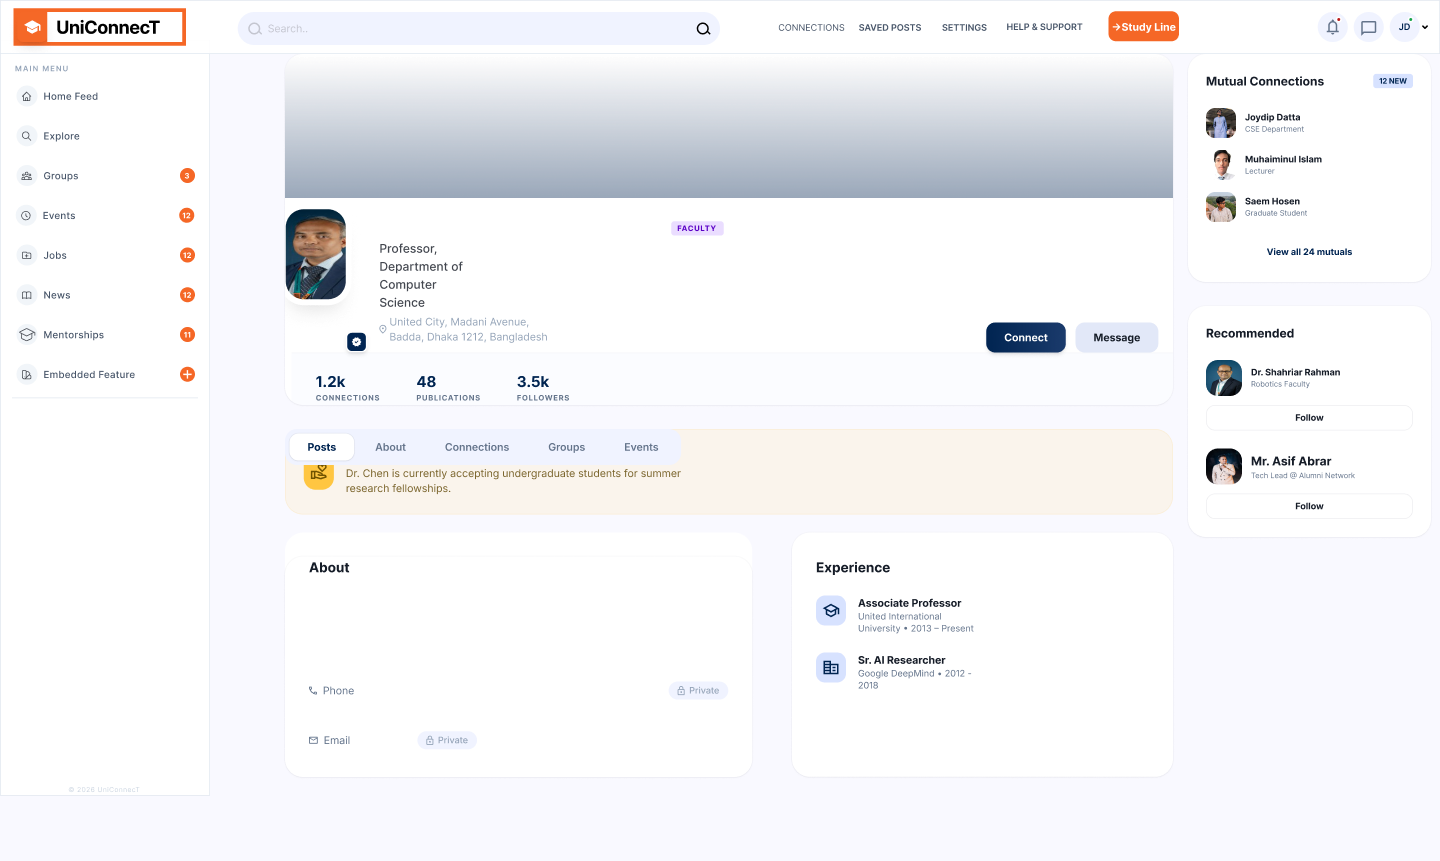
\includegraphics[width=0.85\textwidth, height=0.68\textheight, keepaspectratio]{figma_profile_page.png}
    \caption{Figma Wireframe --- Profile Page. Cover photo, avatar, bio, experience,
    education, skills, featured items, and profile analytics. Edit controls are
    visible for the profile owner.}
    \label{fig:profile}
\end{figure}

% --- Jobs Page ---
\begin{figure}[H]
    \centering
    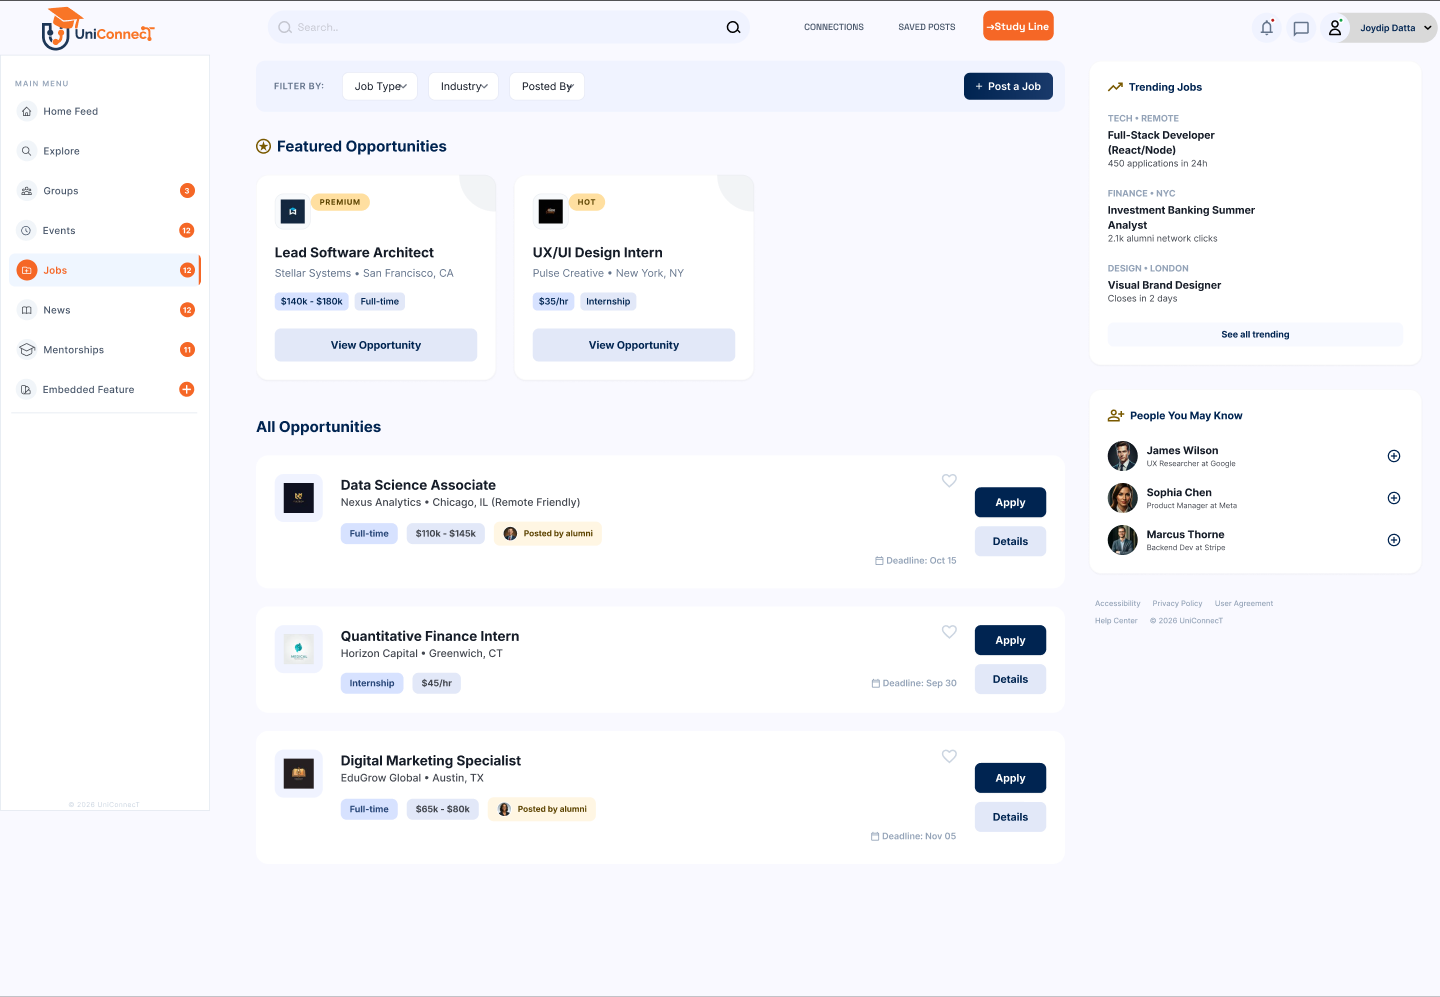
\includegraphics[width=0.85\textwidth, height=0.68\textheight, keepaspectratio]{figma_jobs_page.png}
    \caption{Figma Wireframe --- Jobs Page. Filterable and sortable listing of
    university-internal job and internship postings, with a detail panel for the
    selected listing.}
    \label{fig:jobs}
\end{figure}

% --- Events Page ---
\begin{figure}[H]
    \centering
    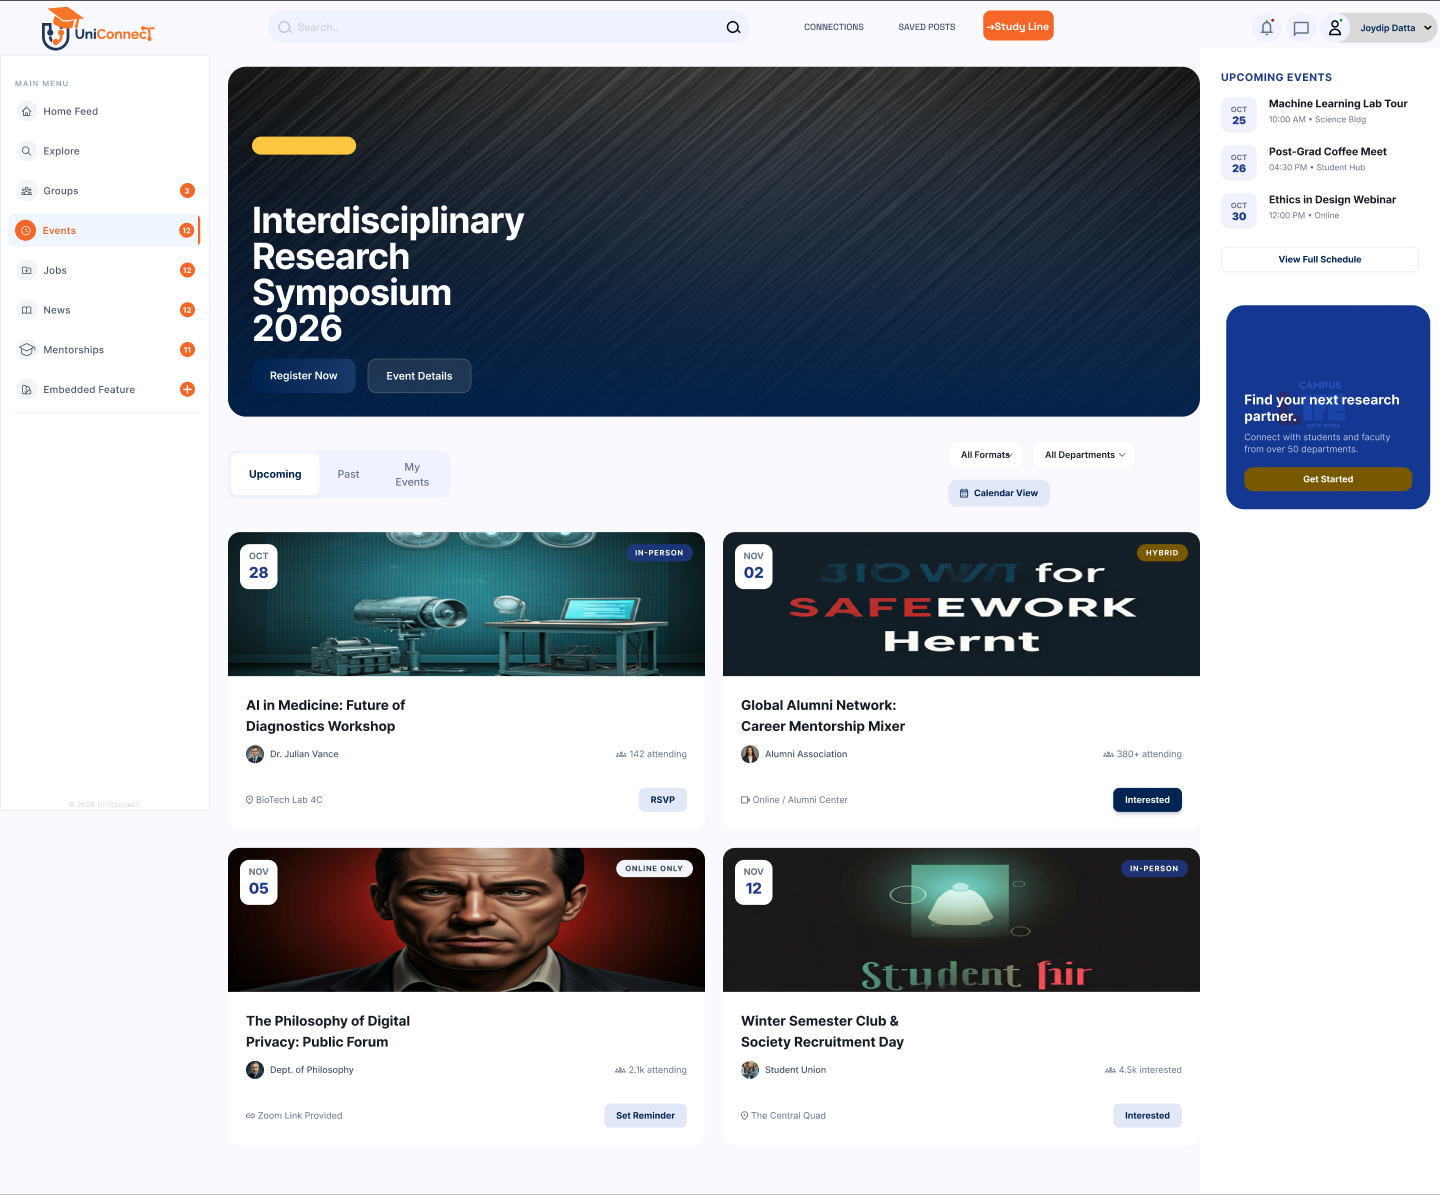
\includegraphics[scale=0.25, keepaspectratio]{figma_events_page.png}
    \caption{Figma Wireframe --- Events Page. Campus event listing with RSVP buttons
    and a detail view showing event date, location, description, and attendee count.}
    \label{fig:events}
\end{figure}

% --- Groups Page ---
\begin{figure}[H]
    \centering
    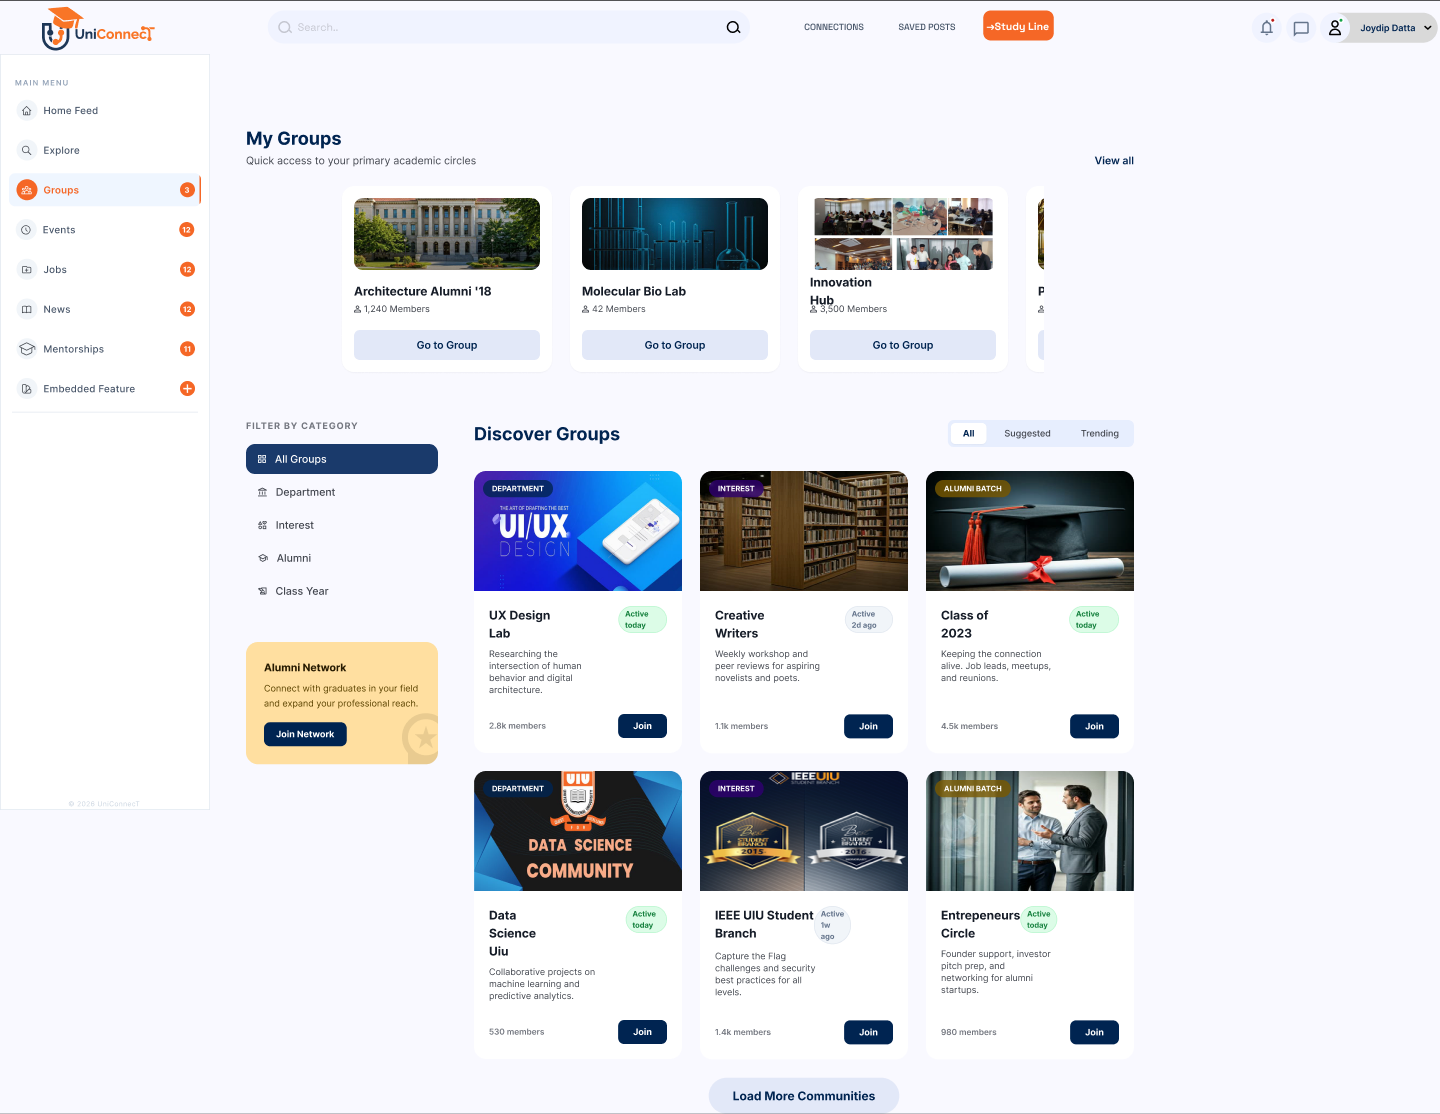
\includegraphics[width=0.85\textwidth, height=0.68\textheight, keepaspectratio]{figma_groups_page.png}
    \caption{Figma Wireframe --- Groups Page. Group directory and a group detail view
    showing the group feed, members list, file resources, study sessions, pinned
    posts, and group rules.}
    \label{fig:groups}
\end{figure}

% --- Messages Page ---
\begin{figure}[H]
    \centering
    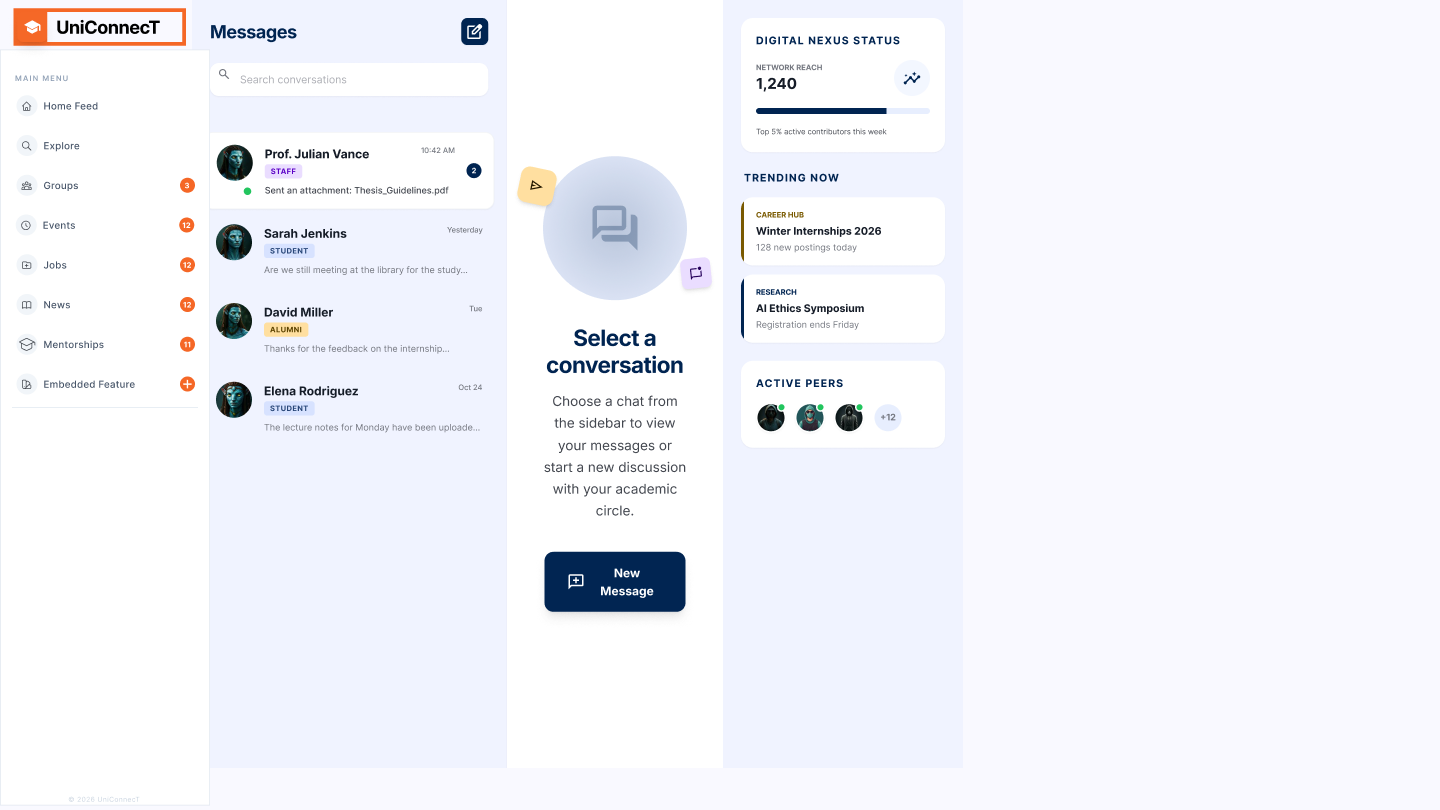
\includegraphics[width=0.85\textwidth, height=0.68\textheight, keepaspectratio]{figma_messages_page.png}
    \caption{Figma Wireframe --- Messages Page. Real-time messaging interface with a
    conversation list on the left and an active chat panel on the right, supporting
    direct messages, group chats, and mentorship threads.}
    \label{fig:messages}
\end{figure}

% --- Mentorship Page ---
\begin{figure}[H]
    \centering
    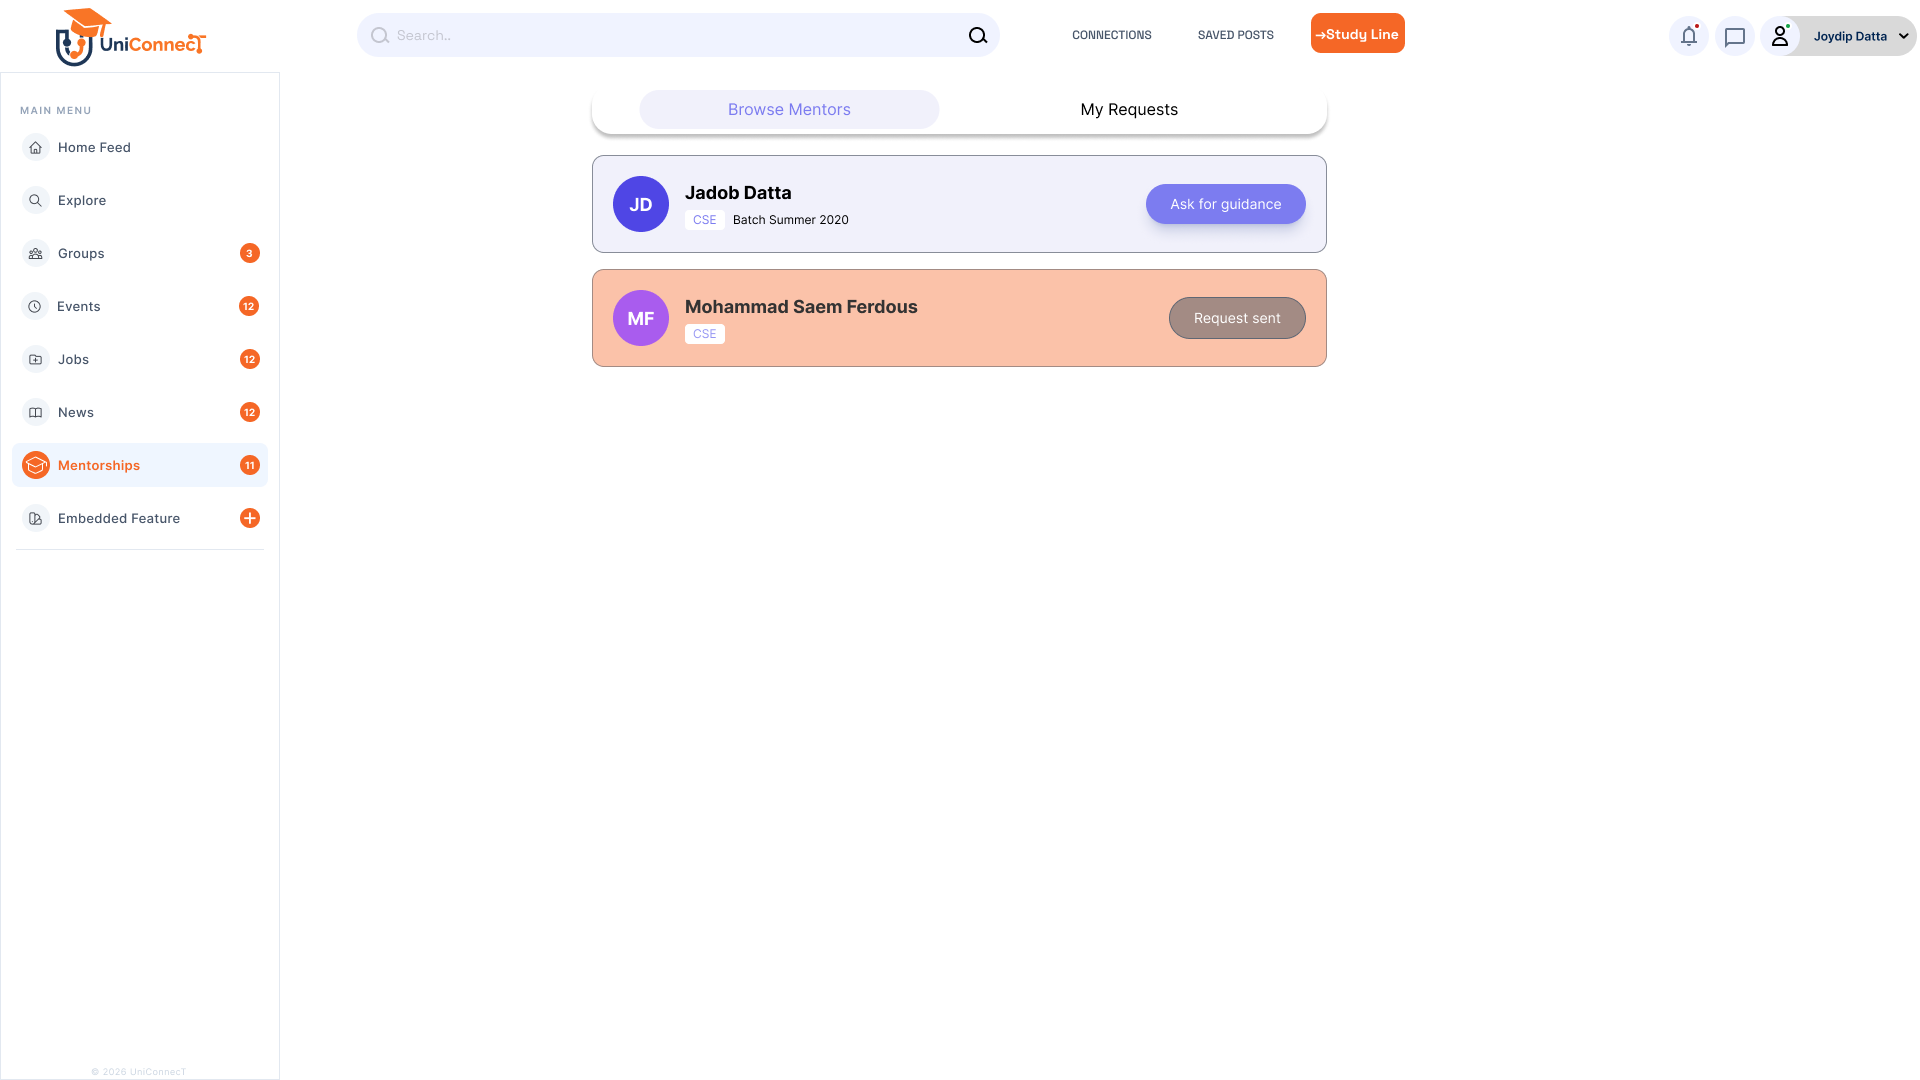
\includegraphics[width=0.85\textwidth, height=0.68\textheight, keepaspectratio]{Mentorship Browse (Student).png}
    \caption{Figma Wireframe --- Mentorship Page. Students browse alumni mentor cards
    and submit requests; alumni manage active mentees, session records, and mentee
    capacity.}
    \label{fig:mentorship}
\end{figure}

\subsection{Campus Utilities and Administration}

% --- Lost and Found + Shuttle ---
\begin{figure}[H]
    \centering
    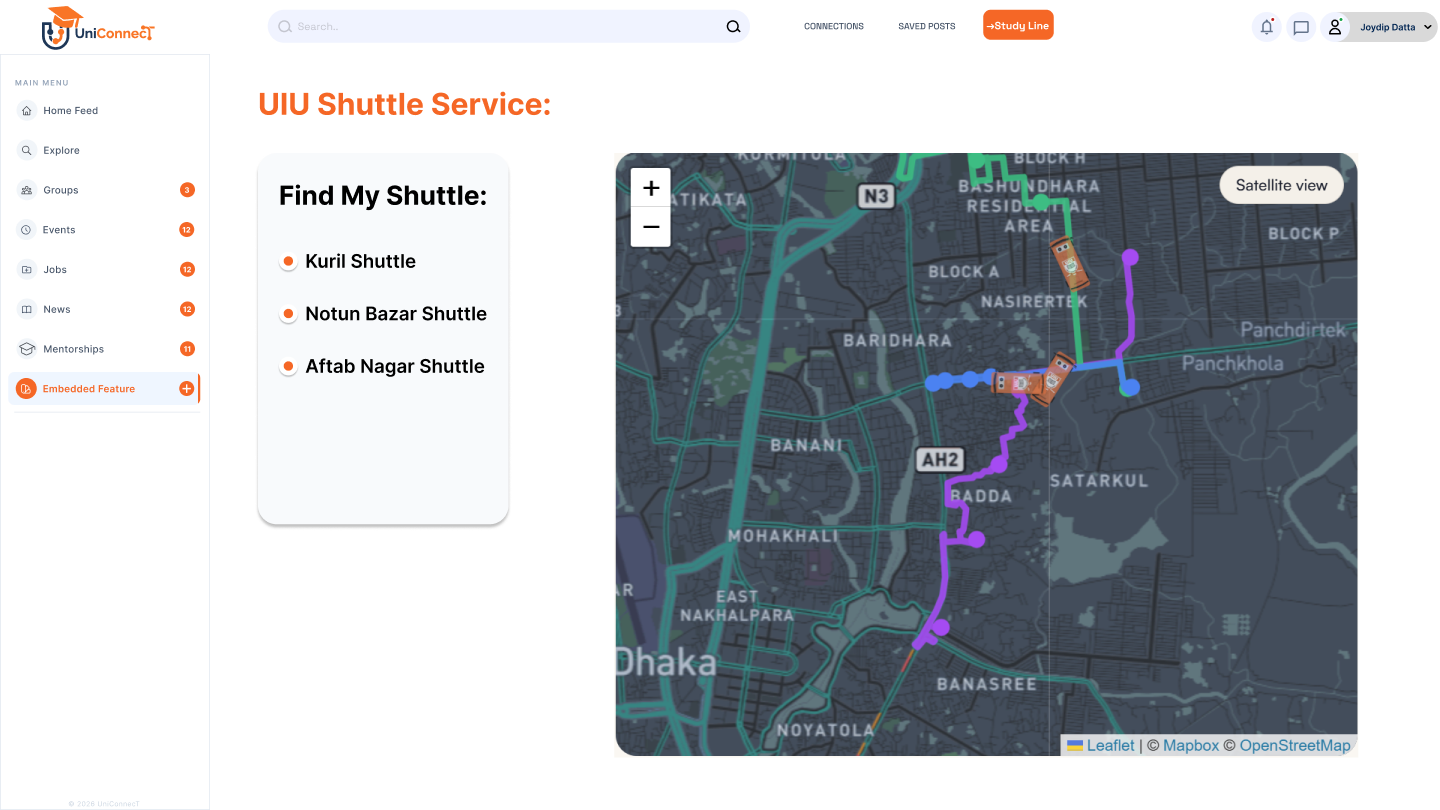
\includegraphics[width=0.85\textwidth, height=0.68\textheight, keepaspectratio]{figma_campus_tools.png}
    \caption{Figma Wireframe --- Shuttle Tracker. The UIU Shuttle Service screen
    lists available shuttle routes (Kuril Shuttle, Notun Bazar Shuttle, Aftab Nagar
    Shuttle) on the left panel, with a live interactive map of the Dhaka route network
    on the right. Students can track real-time shuttle positions directly from this view.}
    \label{fig:campus}
\end{figure}

% --- Admin Panel ---
\begin{figure}[H]
    \centering
    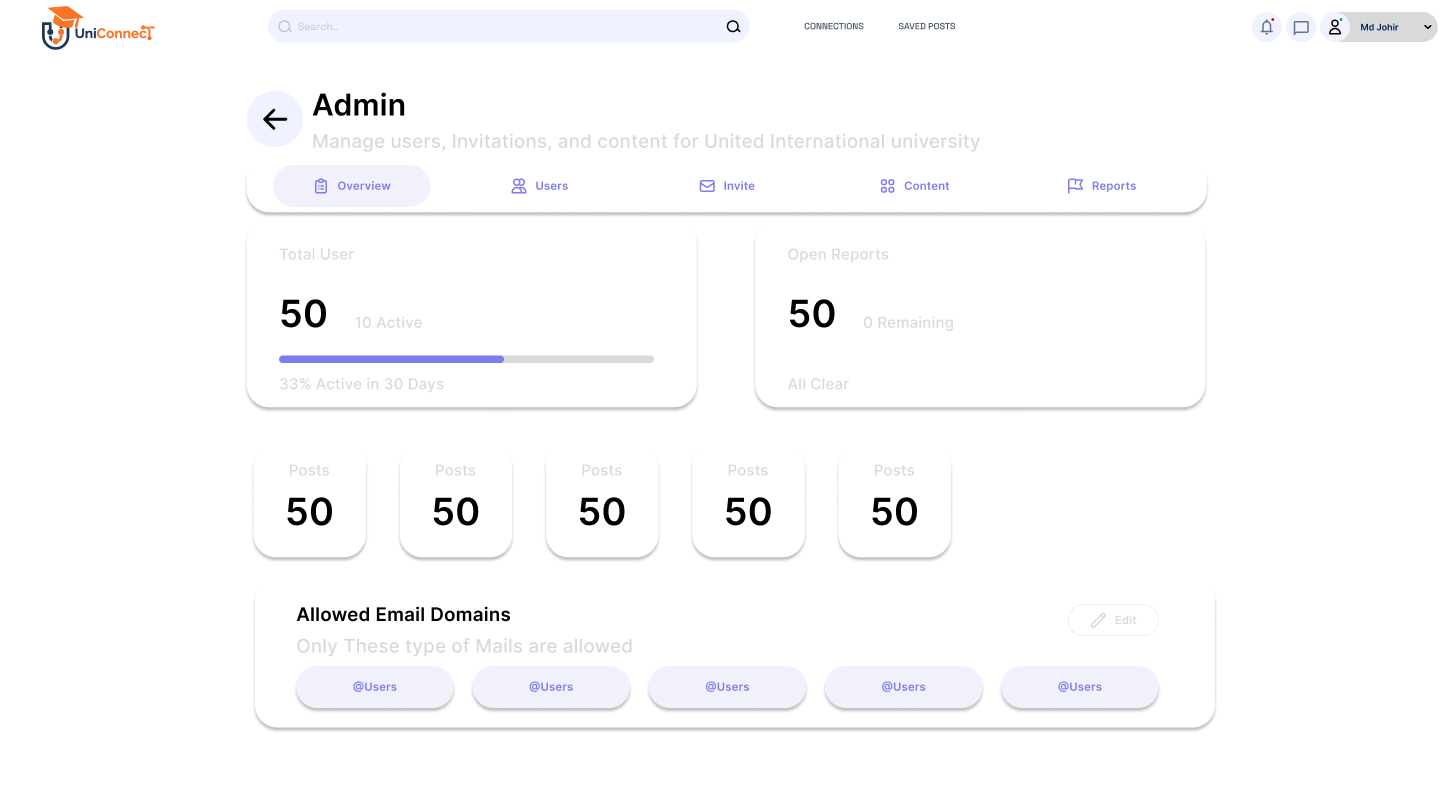
\includegraphics[width=0.85\textwidth, height=0.68\textheight, keepaspectratio]{figma_admin_panel.png}
    \caption{Figma Wireframe --- Admin Panel. Role-restricted management interface
    covering user management, invitation management, content report resolution,
    platform statistics, and university configuration.}
    \label{fig:admin}
\end{figure}

\subsection{System Architecture Diagrams}

% --- Navigation Flow Diagram ---
\begin{figure}[H]
    \centering
    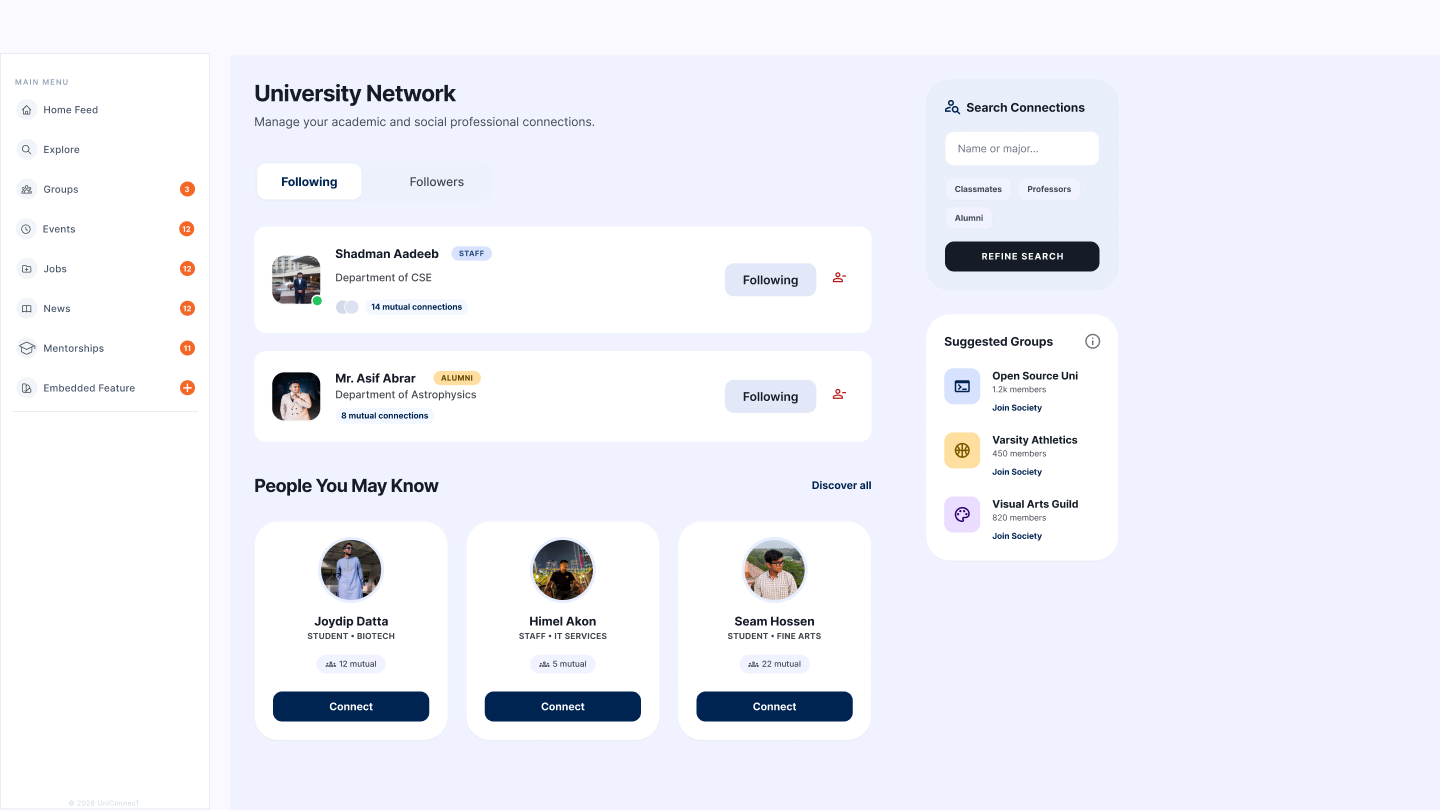
\includegraphics[width=\textwidth, height=0.68\textheight, keepaspectratio]{figma_navigation_flow.png}
    \caption{Figma Wireframe --- University Network (Connections) Page. Displays the
    user's Following and Followers tabs, a ``People You May Know'' section with
    mutual-connection counts and Connect actions, and a right-side panel for searching
    connections by name or major and discovering suggested groups.}
    \label{fig:navflow}
\end{figure}

% --- Module Architecture Diagram ---
\begin{figure}[H]
    \centering
    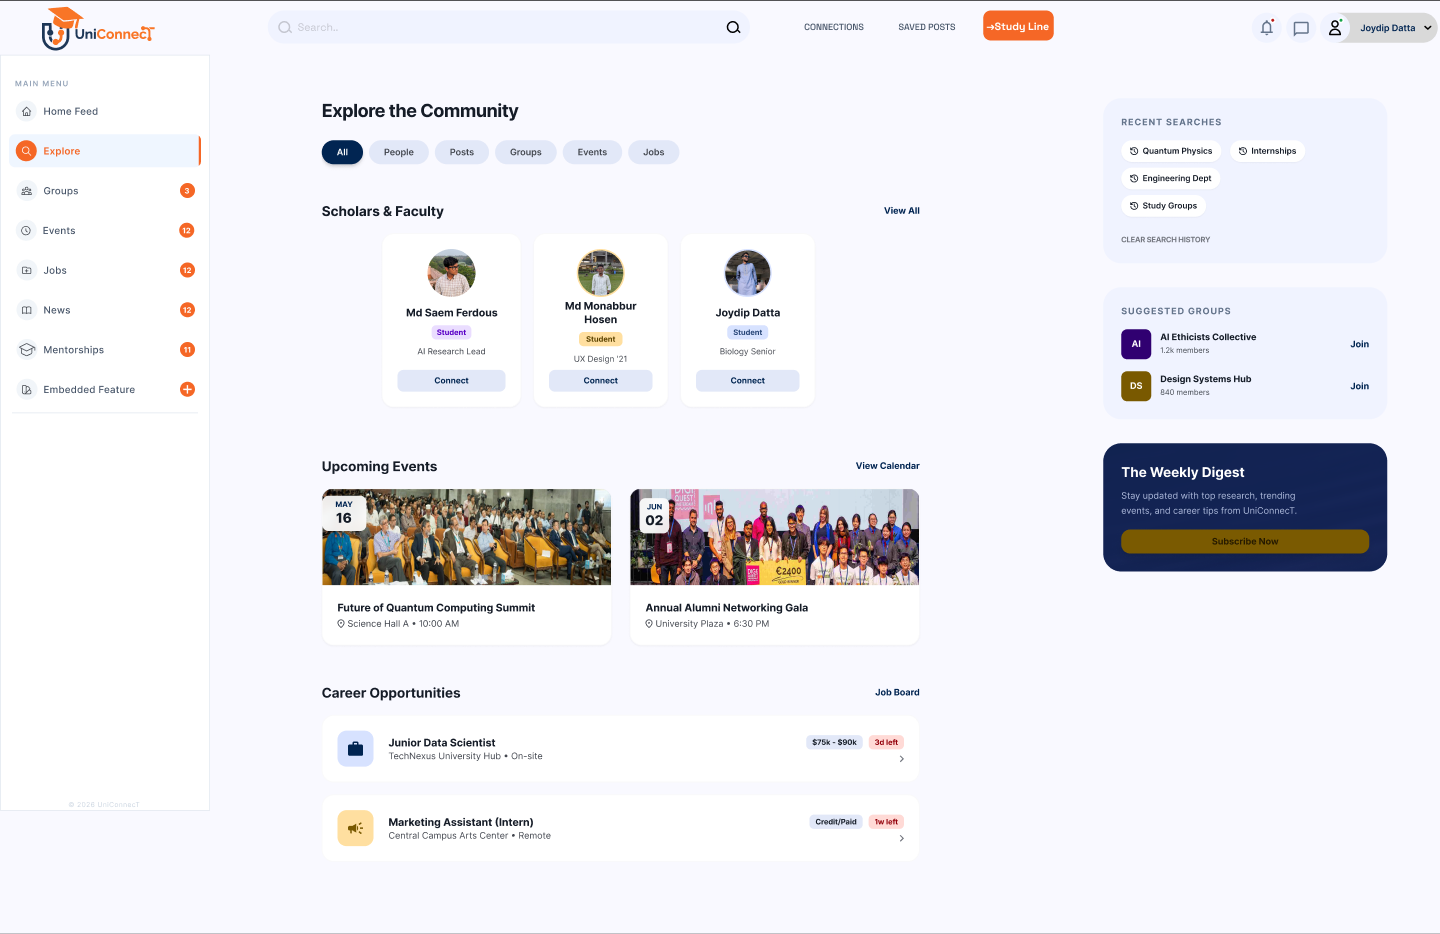
\includegraphics[width=\textwidth, height=0.68\textheight, keepaspectratio]{figma_page_architecture.png}
    \caption{Figma Wireframe --- Explore Page. Surfaces community-wide discovery
    content: a Scholars \& Faculty spotlight with connection actions, Upcoming Events
    with dates and venues, and Career Opportunities pulled from the job board. Filter
    tabs (All, People, Posts, Groups, Events, Jobs) and a right-side panel showing
    Recent Searches and Suggested Groups complete the discovery experience.}
    \label{fig:architecture}
\end{figure}
\clearpage
% ---------------------------------------------------------------
\section{Usability / Design Considerations}
% ---------------------------------------------------------------

\subsection{Navigation Flow}

UniConnecT uses a persistent top navigation bar on all authenticated pages, providing
direct access to the five primary sections: Feed, Jobs, Events, Messages, and
Notifications. A left-side profile summary panel on wider screens offers quick links
to Profile, Groups, Mentorship, Explore, Lost \& Found, Shuttle, and Drafts. The
navigation set is role-aware: admin-only controls (Admin Panel) appear only for
administrator-role users, and the Driver GPS Broadcast View is exclusive to the
driver role. The unauthenticated shell (Landing, Login, Register, OTP, Forgot
Password) is entirely separate from the authenticated application and shares no
navigation elements with it.

\subsection{Responsiveness Across Devices}

The design targets three primary breakpoints: mobile (360px--767px), tablet
(768px--1023px), and desktop (1024px and above). On mobile, the top navigation bar
collapses to a bottom tab bar covering the five primary sections, and the three-column
feed layout (feed + two sidebars) reflows to a single-column view. Job and event card
grids reflow from three columns on desktop to two on tablet and one on mobile. All
interactive touch targets are designed at a minimum of 44$\times$44px on mobile to
meet accessibility touch-target guidelines.

\subsection{Color Consistency and Design System}

UniConnecT is designed with two themes defined in a centralized Figma design system:

\begin{itemize}
    \item \textbf{Warm Futuristic Dark (Default):} Deep navy background surfaces,
    UIU orange as the primary brand and interactive accent, and indigo for secondary
    interactive states. Warm white text tokens are used on all dark surfaces. Coloured
    surfaces (e.g., orange notification badges) use the matching light token for text.

    \item \textbf{Warm Neutral Light:} Off-white and warm grey surfaces with the same
    UIU orange accent, designed for users who prefer a light interface. Toggled via the
    user's theme preference in Settings.
\end{itemize}

No ad-hoc or hardcoded color values appear anywhere in the design. All fills and
strokes reference named Figma color styles. Structural borders are 0.5px. All
buttons use pill-shaped (fully rounded) border radii exclusively.

\subsection{Accessibility Considerations}

\begin{itemize}
    \item \textbf{Color Contrast:} All text-on-background color pairings in both
    themes meet a minimum 4.5:1 contrast ratio (WCAG 2.1 Level AA), verified using
    the A11y Figma plugin during the design process.

    \item \textbf{Typography:} Body text is set at 14px minimum. Font weight is
    restricted to 400 (regular) and 500 (medium) throughout. Section headings
    establish hierarchy through size differences, not color or weight extremes.

    \item \textbf{Interactive States:} All buttons, links, form fields, navigation
    items, and cards include clearly visible hover, focus, and active states, ensuring
    keyboard and screen-reader users can navigate effectively.

    \item \textbf{Labels and Tooltips:} All form inputs carry visible text labels.
    Icon-only controls (e.g., reaction buttons, share, bookmark) include tooltips to
    communicate purpose without relying solely on icon recognition.

    \item \textbf{Empty and Error States:} Every list, feed, and search result view
    has a designed empty state with a clear message. Every form includes inline error
    messages positioned adjacent to the failing field rather than at the top of the
    page only.
\end{itemize}

\subsection{Key User-Friendly Design Decisions}

\begin{itemize}
    \item \textbf{Skeleton Loading States:} The feed, profile, jobs, events, and
    groups pages use skeleton placeholder cards while content loads, ensuring the
    interface never presents a blank screen and conveys immediate responsiveness.

    \item \textbf{Role-Aware Navigation:} Navigation surfaces adapt automatically
    based on the logged-in user's role, so students never encounter admin controls
    and drivers see only their broadcast interface.

    \item \textbf{Progressive Disclosure:} Secondary and advanced actions (post
    editing options, advanced group settings, mentorship session notes, privacy
    controls) are revealed via dropdown menus or modals, keeping primary page views
    uncluttered and focused.

    \item \textbf{Unified Search:} A single persistent search bar in the top
    navigation queries all content types simultaneously, with tabbed result views
    for People, Posts, Jobs, Events, Groups, and News --- removing the need for
    users to navigate to individual sections to search within them.

    \item \textbf{Automatic Mentorship Thread:} When a mentorship request is
    accepted, a dedicated conversation thread is automatically created and surfaced
    in the Messages module, eliminating the friction of manually initiating contact
    after acceptance.

    \item \textbf{Drafts Across Content Types:} A unified Drafts page aggregates
    all of a user's unpublished content (posts, jobs, news, events) in one place,
    preventing work from being lost across disconnected creation flows.

    \item \textbf{Consistent Component Language:} Cards, modals, input fields,
    badges, tabs, and buttons follow a single visual specification across all 24
    pages of the design, reducing the visual learning curve for new users and
    ensuring a coherent, professional-quality interface throughout.
\end{itemize}

% ---------------------------------------------------------------
\clearpage
\section{Conclusion}
% ---------------------------------------------------------------

UniConnecT is a planned private university social networking platform designed to
address the fragmentation and absence of a dedicated digital community space for
university students, alumni, faculty, and staff. This Software Requirements
Specification documents the system's five intended user roles, 29 functional
requirements spanning social networking, professional development, mentorship, campus
utilities, real-time communication, and administration, 10 non-functional quality
requirements, and the full scope of 24 planned pages and modules --- all expressed
through the UniConnecT Figma design prototype.

The design goals of UniConnecT center on delivering a unified, role-aware, and
accessible platform that connects every member of the university community in a single
trusted environment. By grounding the design in a coherent UIU-branded design system
(Warm Futuristic Dark and Warm Neutral Light themes), a clear multi-role navigation
architecture, and established WCAG 2.1 accessibility standards, the planned interface
is intended to provide a modern, student-centric experience that meaningfully bridges
academic life, professional development, and everyday campus engagement.

This SRS, prepared by Team Mavericks as part of the System Analysis and Design course
at United International University (UIU), serves as the foundational specification for
the accompanying Figma prototype and guides all design decisions made throughout the
project.

% ---------------------------------------------------------------
\end{document}
